\documentclass[12pt,a4paper]{article}
\usepackage[a4paper, margin=0.8in, headheight=14pt]{geometry}
\usepackage{fontspec}
\usepackage{unicode-math}
\setmainfont{TeX Gyre Pagella}
\setmonofont[Scale=0.88]{TeX Gyre Cursor}
\setmathfont{Latin Modern Math}
\usepackage{xcolor}
\usepackage{titlesec}
\usepackage{enumitem}
\usepackage{tabularx}
\usepackage{booktabs}
\usepackage{array}
\usepackage{amsmath}
\usepackage{tikz}
\usetikzlibrary{shapes.geometric, arrows.meta, positioning, calc, fit, decorations.pathreplacing}
\usepackage{tcolorbox}
\tcbuselibrary{skins, breakable}
\usepackage{hyperref}
\usepackage{fancyhdr}
\usepackage{graphicx}
\usepackage{microtype}
\hyphenpenalty=10000
\exhyphenpenalty=10000
\sloppy
\usepackage{caption}
\usepackage{setspace}
\usepackage{multirow}
\usepackage{tocloft}
\newcommand{\Q}[1]{\textbf{#1}\par\noindent\ignorespaces}
\definecolor{myred}{RGB}{196,30,58}
\definecolor{mydark}{RGB}{30,30,50}
\definecolor{mygreen}{RGB}{14,120,80}
\definecolor{myteal}{RGB}{0,130,140}
\definecolor{myamber}{RGB}{180,100,0}
\definecolor{mypurple}{RGB}{100,30,160}
\definecolor{mygray}{RGB}{246,247,249}
\definecolor{mgframe}{RGB}{180,185,200}
\definecolor{watermark}{RGB}{145,150,170}
\definecolor{hdrred}{RGB}{250,232,235}
\definecolor{hdrgreen}{RGB}{220,244,233}
\definecolor{hdrteal}{RGB}{220,242,244}
\definecolor{hdramber}{RGB}{253,242,215}
\definecolor{hdrpurple}{RGB}{238,228,255}
\definecolor{hdrgray}{RGB}{238,240,245}
\definecolor{rowalt}{RGB}{250,251,253}

\titleformat{\section}{\large\bfseries\color{myred}}{\thesection.}{0.5em}{}[\vspace{1pt}{\color{myred}\rule{\linewidth}{0.8pt}}]
\titleformat{\subsection}{\normalsize\bfseries\color{myteal}}{\thesubsection}{0.5em}{}
\titlespacing*{\section}{0pt}{18pt}{7pt}
\titlespacing*{\subsection}{0pt}{11pt}{4pt}
\setlength{\parindent}{0pt}
\setlength{\parskip}{4pt}
\renewcommand{\cfttoctitlefont}{\large\bfseries\color{myred}}
\renewcommand{\cftaftertoctitle}{\par\noindent{\color{myred}\rule{\linewidth}{0.8pt}}}
\setlength{\cftbeforetoctitleskip}{0pt}
\setlength{\cftaftertoctitleskip}{6pt}
\renewcommand{\cftsecfont}{\normalsize\bfseries\color{mydark}}
\renewcommand{\cftsecpagefont}{\normalsize\bfseries\color{mydark}}
\renewcommand{\cftsecleader}{\cftdotfill{\cftdotsep}}
\setlength{\cftbeforesecskip}{7pt}
\renewcommand{\cftsubsecfont}{\small\color{mydark}}
\renewcommand{\cftsubsecpagefont}{\small\color{mydark}}
\setlength{\cftbeforesubsecskip}{3pt}
\setlength{\cftsubsecindent}{1.4em}
\renewcommand{\cftpartfont}{\normalsize\bfseries\color{myteal}}
\renewcommand{\cftpartpagefont}{\normalsize\bfseries\color{myteal}}
\setlength{\cftbeforepartskip}{14pt}
\renewcommand{\arraystretch}{1.45}
\setlength{\tabcolsep}{6pt}
\newcolumntype{B}[1]{>{\small\bfseries\raggedright\arraybackslash}m{#1}}
\newcolumntype{C}[1]{>{\centering\arraybackslash}m{#1}}
\newcolumntype{Y}{>{\small\raggedright\arraybackslash}X}
\renewcommand{\tabularxcolumn}[1]{m{#1}}
\newcommand{\currmodule}{Module 1}
\pagestyle{fancy}
\fancyhf{}
\fancyhead[L]{\small\color{myred}\textbf{EC602}\;\color{mydark}--- Computer Network}
\fancyhead[R]{\small\color{myteal}\textbf{\currmodule\ Notes}}
\fancyfoot[C]{\small\color{mydark}\thepage}
\fancyfoot[R]{\small\color{watermark}\textit{\copyright\ Biraj}}
\renewcommand{\headrulewidth}{0.5pt}
\renewcommand{\footrulewidth}{0.3pt}

\hypersetup{colorlinks=true, linkcolor=myteal, urlcolor=myteal,
  pdfauthor={Biraj Sarkar},
  pdftitle={EC602 --- Combined Notes}}

\tcbset{
  tikzbox/.style={
    colback=mygray, colframe=mgframe, boxrule=0.6pt, arc=4pt,
    left=8pt, right=8pt, top=6pt, bottom=6pt,
    colbacktitle=mgframe, coltitle=mydark,
    fonttitle=\small\bfseries
  },
  defbox/.style={
    colback=hdrgreen, colframe=mygreen, boxrule=0.8pt, arc=4pt,
    left=9pt, right=9pt, top=6pt, bottom=6pt,
    colbacktitle=mygreen, coltitle=white,
    fonttitle=\small\bfseries
  },
  formulabox/.style={
    colback=hdrteal, colframe=myteal, boxrule=0.8pt, arc=4pt,
    left=9pt, right=9pt, top=7pt, bottom=7pt,
    colbacktitle=myteal, coltitle=white,
    fonttitle=\small\bfseries
  },
  examplebox/.style={
    colback=hdramber, colframe=myamber, boxrule=0.8pt, arc=4pt,
    left=9pt, right=9pt, top=6pt, bottom=6pt,
    colbacktitle=myamber, coltitle=white,
    fonttitle=\small\bfseries
  },
  masonbox/.style={
    colback=hdrpurple, colframe=mypurple, boxrule=0.8pt, arc=4pt,
    left=9pt, right=9pt, top=6pt, bottom=6pt,
    colbacktitle=mypurple, coltitle=white,
    fonttitle=\small\bfseries
  },
  exambox/.style={
    colback=hdrpurple, colframe=mypurple, boxrule=1pt, arc=5pt,
    left=10pt, right=10pt, top=8pt, bottom=8pt,
    colbacktitle=mypurple, coltitle=white,
    fonttitle=\bfseries,
    breakable
  }
}
\tcbset{breakable}

\tikzset{
  block/.style={rectangle, draw=myteal, fill=hdrteal,
    text width=2.4cm, align=center, minimum height=0.95cm,
    font=\small, rounded corners=3pt, line width=0.7pt},
  redblock/.style={rectangle, draw=myred, fill=hdrred,
    text width=2.4cm, align=center, minimum height=0.95cm,
    font=\small, rounded corners=3pt, line width=0.7pt},
  netnode/.style={rectangle, draw=myteal, fill=hdrteal,
    text width=1.5cm, align=center, minimum height=0.8cm,
    font=\small, rounded corners=3pt, line width=0.7pt},
  arrow/.style={-Stealth, thick, color=mydark},
  redarrow/.style={-Stealth, thick, color=myred},
  line/.style={thick, color=mydark}
}

\newcommand{\modulestart}[2]{%
  \clearpage
  \renewcommand{\currmodule}{Module #1}%
  \phantomsection
  \addcontentsline{toc}{part}{Module #1: #2}%
  \setcounter{section}{0}%
  \begin{center}
    \vspace*{1.0cm}
    {\Huge\bfseries\color{myred} Module #1}\\[10pt]
    {\Large\bfseries\color{mydark} #2}\\[10pt]
    {\color{myred}\rule{0.55\linewidth}{1.2pt}}
  \end{center}
  \vspace{14pt}
}
\begin{document}

\thispagestyle{empty}
\vspace*{1.0cm}
\begin{center}
  {\Huge\bfseries\color{myred} EC602}\\[10pt]
  {\LARGE\bfseries\color{mydark} Computer Network}\\[20pt]
  {\color{myred}\rule{0.7\linewidth}{1.5pt}}\\[18pt]
  {\Large\color{myteal}\textbf{Combined Module Notes}}\\[8pt]
  {\large\color{mydark} Modules 1 -- 4}\\[40pt]
  {\normalsize\color{mydark} Semester VI \quad$\bullet$\quad 3L:0T:0P \quad$\bullet$\quad 3 Credits}\\[12pt]
  {\normalsize\color{mydark} CGEC \;$|$\; B.Tech ECE (2023--27)}\\[6pt]
  {\normalsize\color{mydark}\textit{Biraj Sarkar}}
\end{center}
\vspace{1.0cm}
\begin{center}
  \begin{tcolorbox}[colback=mygray, colframe=mgframe, boxrule=0.5pt, arc=3pt, width=0.85\linewidth]
    \centering\small\color{mydark}
    \textbf{Disclaimer / Study Guide Notice:}\\
    These are condensed \textbf{Short Notes} focusing on core theory, key formulas, block/circuit diagrams, and standard viva Q\&As for university exam revision. Exhaustive numerical practice problems and derivation edge cases are not covered. This serves as a quick-revision reference guide for students.
  \end{tcolorbox}
\end{center}
\vfill
\begin{center}{\small\color{watermark}\textit{Exam-Ready Notes}}\end{center}
\clearpage

\hypersetup{linkcolor=mydark}
\tableofcontents
\hypersetup{linkcolor=myteal}
\clearpage

% -- Module 1 -----------------------------------------------------------------
\modulestart{1}{Overview of Data Communication and Networking}

\section{Overview of Data Communication and Networking}
%═══════════════════════════════════════════════════════════════════════════════

\begin{tcolorbox}[defbox]
\textbf{Data Communication:} The exchange of data between two devices via a transmission medium. It requires a \textit{sender}, \textit{receiver}, \textit{message}, \textit{medium}, and \textit{protocol}.
\end{tcolorbox}

\subsection{Components of Data Communication}

\begin{tabularx}{\linewidth}{|B{3.2cm}|X|}
\hline
\multicolumn{1}{|>{\centering\arraybackslash}p{3.2cm}|}{\textbf{\color{mygreen}Component}} &
\multicolumn{1}{>{\centering\arraybackslash}X|}{\textbf{\color{mygreen}Description}} \\
\hline
Message        & The information (data) to be communicated --- text, numbers, images, audio, video. \\
\hline
Sender         & The device that sends the data message (computer, phone, camera). \\
\hline
Receiver       & The device that receives the message (computer, printer, phone). \\
\hline
Medium         & The physical path over which the message travels (cable, air, fibre). \\
\hline
Protocol       & A set of rules governing data communication; ensures sender and receiver agree on format, timing, and error handling. \\
\hline
\end{tabularx}

\subsection{Data Representation}

Data is represented in different formats depending on the type of information:\par\noindent
\begin{tabularx}{\linewidth}{|B{3.0cm}|X|}
\hline
\multicolumn{1}{|>{\centering\arraybackslash}p{3.0cm}|}{\textbf{\color{myteal}Type}} &
\multicolumn{1}{>{\centering\arraybackslash}X|}{\textbf{\color{myteal}Representation}} \\
\hline
Text           & Encoded using bit patterns --- \textbf{ASCII} (7-bit, 128 chars), \textbf{ISO 8859} (8-bit, 256 chars), \textbf{Unicode} (32-bit, universal). \\
\hline
Numbers        & Stored directly in binary; not converted to ASCII to save space. \\
\hline
Images         & Represented as a matrix of pixels; each pixel encoded in bits (RGB). \\
\hline
Audio          & Continuous signal sampled at regular intervals and quantised to binary values. \\
\hline
Video          & Sequence of images (frames) displayed at a rate (fps) to create motion. \\
\hline
\end{tabularx}

\subsection{Direction of Data Flow}

\begin{tcolorbox}[tikzbox, title={Data Flow Modes}]
\centering
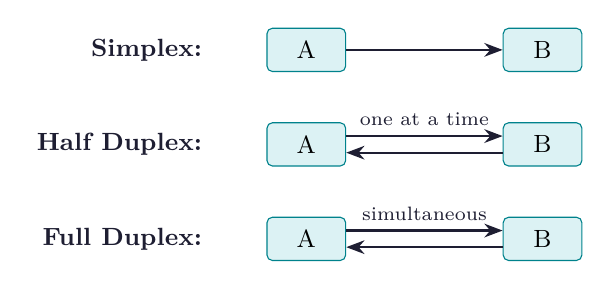
\begin{tikzpicture}[
  dev/.style={rectangle, draw=myteal, fill=hdrteal, minimum width=1.0cm, minimum height=0.55cm, align=center, font=\small, rounded corners=2pt},
  lbl/.style={font=\small\bfseries\color{mydark}, anchor=east}
]
% Simplex
\node[lbl] at (0, 3.0) {Simplex:};
\node[dev] (SA) at (1.2, 3.0) {A};
\node[dev] (SB) at (4.2, 3.0) {B};
\draw[arrow] (SA) -- (SB);

% Half Duplex
\node[lbl] at (0, 1.8) {Half Duplex:};
\node[dev] (HA) at (1.2, 1.8) {A};
\node[dev] (HB) at (4.2, 1.8) {B};
\draw[arrow] ([yshift=3pt]HA.east) -- node[above, font=\scriptsize] {one at a time} ([yshift=3pt]HB.west);
\draw[arrow] ([yshift=-3pt]HB.west) -- ([yshift=-3pt]HA.east);

% Full Duplex
\node[lbl] at (0, 0.6) {Full Duplex:};
\node[dev] (FA) at (1.2, 0.6) {A};
\node[dev] (FB) at (4.2, 0.6) {B};
\draw[arrow] ([yshift=3pt]FA.east) -- node[above, font=\scriptsize] {simultaneous} ([yshift=3pt]FB.west);
\draw[arrow] ([yshift=-3pt]FB.west) -- ([yshift=-3pt]FA.east);
\end{tikzpicture}
\end{tcolorbox}

\begin{tabularx}{\linewidth}{|B{3.0cm}|X|X|}
\hline
\multicolumn{1}{|>{\centering\arraybackslash}p{3.0cm}|}{\textbf{Mode}} &
\multicolumn{1}{>{\centering\arraybackslash}X|}{\textbf{Description}} &
\multicolumn{1}{>{\centering\arraybackslash}X|}{\textbf{Example}} \\
\hline
Simplex        & One direction only; receiver cannot send back. & TV broadcast, keyboard to CPU \\
\hline
Half Duplex    & Both directions, but \textbf{not simultaneously}; one at a time. & Walkie-talkie, CB radio \\
\hline
Full Duplex    & Both directions \textbf{simultaneously}; uses two separate channels or frequencies. & Telephone, mobile call \\
\hline
\end{tabularx}

\subsection{Network Criteria}

A good network must satisfy three fundamental criteria:

\begin{tcolorbox}[formulabox, title={\textbf{Three Criteria of a Good Network}}]
\begin{enumerate}[label=\textbf{\arabic*.}, leftmargin=*, itemsep=4pt, topsep=0pt]
  \item \textbf{Performance} --- measured by transit time (time for a message to travel from sender to receiver) and response time. Affected by number of users, type of medium, hardware, and software.
  \item \textbf{Reliability} --- frequency of failure, recovery time after failure, robustness in catastrophe.
  \item \textbf{Security} --- protecting data from unauthorised access, damage, and implementing recovery policies.
\end{enumerate}
\end{tcolorbox}

%═══════════════════════════════════════════════════════════════════════════════
\section{Physical Structure: Topology and Categories}
%═══════════════════════════════════════════════════════════════════════════════

\subsection{Network Topologies}

\begin{tcolorbox}[defbox]
\textbf{Topology:} The geometric arrangement of devices (nodes) and links in a network. It defines how devices are physically or logically connected.
\end{tcolorbox}

\begin{tcolorbox}[tikzbox, title={Common Network Topologies}]
\centering
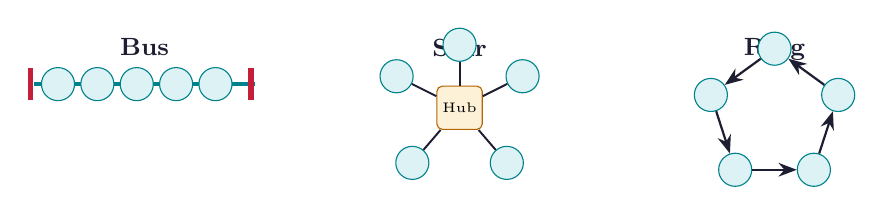
\begin{tikzpicture}[
  dev/.style={circle, draw=myteal, fill=hdrteal, minimum size=0.42cm, inner sep=0pt},
  hub/.style={rectangle, draw=myamber, fill=hdramber, minimum size=0.55cm, inner sep=2pt, font=\tiny, rounded corners=2pt},
  lbl/.style={font=\small\bfseries\color{mydark}, anchor=north}
]

%--- BUS (left) ---
\node[lbl] at (1.5, 3.2) {Bus};
\draw[line width=1.4pt, color=myteal] (0.1, 2.5) -- (2.9, 2.5);
\foreach \x in {0.4, 0.9, 1.4, 1.9, 2.4} {
  \node[dev] at (\x, 2.5) {};
}
% terminators
\draw[line width=2pt, color=myred] (0.05, 2.3) -- (0.05, 2.7);
\draw[line width=2pt, color=myred] (2.85, 2.3) -- (2.85, 2.7);

%--- STAR (centre) ---
\node[lbl] at (5.5, 3.2) {Star};
\node[hub] (H) at (5.5, 2.2) {Hub};
% 5 devices around hub at fixed positions
\node[dev] (N1) at (5.5, 3.0) {};
\node[dev] (N2) at (6.3, 2.6) {};
\node[dev] (N3) at (6.1, 1.5) {};
\node[dev] (N4) at (4.9, 1.5) {};
\node[dev] (N5) at (4.7, 2.6) {};
\foreach \n in {N1,N2,N3,N4,N5} { \draw[line width=0.7pt, color=mydark] (H) -- (\n); }

%--- RING (right) ---
\node[lbl] at (9.5, 3.2) {Ring};
\foreach \i in {0,1,2,3,4} {
  \pgfmathsetmacro\ang{90 + \i*72}
  \node[dev] (R\i) at ($(9.5, 2.1)+(\ang:0.85cm)$) {};
}
\foreach \i/\j in {0/1,1/2,2/3,3/4,4/0} {
  \draw[-Stealth, thick, color=mydark] (R\i) -- (R\j);
}
\end{tikzpicture}
\end{tcolorbox}

\begin{tabularx}{\linewidth}{|B{2.8cm}|X|X|}
\hline
\multicolumn{1}{|>{\centering\arraybackslash}p{2.8cm}|}{\textbf{Topology}} &
\multicolumn{1}{>{\centering\arraybackslash}X|}{\textbf{Description}} &
\multicolumn{1}{>{\centering\arraybackslash}X|}{\textbf{Advantage / Disadvantage}} \\
\hline
Bus            & All devices share a single backbone cable. Terminators at both ends. & Simple, cheap / Single point of failure; collisions. \\
\hline
Star           & All devices connect to a central hub/switch. & Easy fault isolation / Hub failure = network down. \\
\hline
Ring           & Each device connects to exactly two others forming a closed loop. & Equal access / One break disrupts entire ring. \\
\hline
Mesh           & Every device connects to every other device (full mesh) or some (partial mesh). & Highly reliable / Expensive, complex wiring. \\
\hline
Tree (Hybrid)  & Hierarchical combination of star and bus topologies. & Scalable / Backbone failure affects subtrees. \\
\hline
\end{tabularx}

\subsection{Categories of Networks}

\begin{tabularx}{\linewidth}{|B{2.4cm}|>{\centering\arraybackslash}p{2.8cm}|X|}
\hline
\multicolumn{1}{|>{\centering\arraybackslash}p{2.4cm}|}{\textbf{\color{myteal}Category}} &
\textbf{\color{myteal}Coverage} &
\multicolumn{1}{>{\centering\arraybackslash}X|}{\textbf{\color{myteal}Description \& Examples}} \\
\hline
LAN            & Up to a few km & Local Area Network; single building or campus. Ethernet, Wi-Fi. High speed (100 Mbps--10 Gbps). \\
\hline
MAN            & City-wide (5--50 km) & Metropolitan Area Network; connects multiple LANs in a city. Cable TV networks, WiMAX. \\
\hline
WAN            & Country / Global & Wide Area Network; connects cities, countries. Internet, leased lines, satellite links. \\
\hline
\end{tabularx}

%═══════════════════════════════════════════════════════════════════════════════
\section{Internet: History and Protocols}
%═══════════════════════════════════════════════════════════════════════════════

\begin{tcolorbox}[defbox]
\textbf{Internet:} A global network of networks interconnected using the TCP/IP protocol suite. It evolved from ARPANET (1969), a US Department of Defense project for fault-tolerant communication.
\end{tcolorbox}

\textbf{Brief History:}
\begin{itemize}[leftmargin=*, itemsep=3pt]
  \item \textbf{1969} --- ARPANET launched; first 4-node network (UCLA, Stanford, UCSB, Utah).
  \item \textbf{1974} --- TCP/IP protocol defined by Cerf and Kahn.
  \item \textbf{1983} --- ARPANET officially adopts TCP/IP; modern Internet born.
  \item \textbf{1991} --- World Wide Web (WWW) introduced by Tim Berners-Lee at CERN.
  \item \textbf{1993} --- Mosaic browser; Internet becomes publicly accessible.
\end{itemize}

\textbf{Protocols and Standards:} A \textbf{protocol} is a set of rules governing communication. A \textbf{standard} is a protocol agreed upon by industry bodies. Key bodies: \textbf{ISO}, \textbf{IEEE}, \textbf{IETF}, \textbf{ITU-T}, \textbf{ANSI}.

%═══════════════════════════════════════════════════════════════════════════════
\section{Reference Models}
%═══════════════════════════════════════════════════════════════════════════════

\subsection{OSI Reference Model}

\begin{tcolorbox}[defbox]
\textbf{OSI Model (Open Systems Interconnection):} A 7-layer conceptual framework developed by ISO (1984) to standardise communication between different systems. Each layer has specific functions and communicates with adjacent layers via interfaces.
\end{tcolorbox}

\begin{tabularx}{\linewidth}{|>{\centering\arraybackslash}p{0.6cm}|B{3.0cm}|X|}
\hline
\multicolumn{1}{|>{\centering\arraybackslash}p{0.6cm}|}{\textbf{\color{myteal}\#}} &
\multicolumn{1}{>{\centering\arraybackslash}p{3.0cm}|}{\textbf{\color{myteal}Layer}} &
\multicolumn{1}{>{\centering\arraybackslash}X|}{\textbf{\color{myteal}Function \& PDU}} \\
\hline
7 & Application  & User interface; provides network services to applications. PDU: \textit{Data}. Protocols: HTTP, FTP, SMTP, DNS. \\
\hline
6 & Presentation & Translation, encryption, compression of data. PDU: \textit{Data}. \\
\hline
5 & Session      & Establishes, manages, and terminates sessions between applications. PDU: \textit{Data}. \\
\hline
4 & Transport    & End-to-end delivery, segmentation, flow control, error control. PDU: \textit{Segment}. Protocols: TCP, UDP. \\
\hline
3 & Network      & Logical addressing (IP), routing, path determination. PDU: \textit{Packet}. Protocols: IP, ICMP, RIP, OSPF. \\
\hline
2 & Data Link    & Framing, physical addressing (MAC), error detection, flow control. PDU: \textit{Frame}. Protocols: Ethernet, HDLC. \\
\hline
1 & Physical     & Transmission of raw bits over medium; defines electrical/optical signals. PDU: \textit{Bits}. \\
\hline
\end{tabularx}

\subsection{TCP/IP Reference Model}

\begin{tcolorbox}[defbox]
\textbf{TCP/IP Model:} A 4-layer practical model that forms the basis of the Internet. Developed by the DARPA. Less abstract than OSI; combines OSI layers 5, 6, 7 into Application and layers 1, 2 into Network Access.
\end{tcolorbox}

\begin{tabularx}{\linewidth}{|B{3.2cm}|>{\centering\arraybackslash}p{3.0cm}|X|}
\hline
\multicolumn{1}{|>{\centering\arraybackslash}p{3.2cm}|}{\textbf{\color{myteal}TCP/IP Layer}} &
\textbf{\color{myteal}OSI Equivalent} &
\multicolumn{1}{>{\centering\arraybackslash}X|}{\textbf{\color{myteal}Protocols}} \\
\hline
Application    & Layers 5, 6, 7 & HTTP, FTP, SMTP, DNS, SNMP, Telnet \\
\hline
Transport      & Layer 4        & TCP, UDP \\
\hline
Internet       & Layer 3        & IP (IPv4, IPv6), ICMP, ARP, RARP \\
\hline
Network Access & Layers 1, 2    & Ethernet, Wi-Fi (802.11), Token Ring, Frame Relay \\
\hline
\end{tabularx}

\subsection{OSI vs.\ TCP/IP --- Comparison}

\begin{tabularx}{\linewidth}{|B{3.2cm}|X|X|}
\hline
\multicolumn{1}{|>{\centering\arraybackslash}p{3.2cm}|}{\textbf{Parameter}} &
\multicolumn{1}{>{\centering\arraybackslash}X|}{\textbf{\color{myteal}OSI Model}} &
\multicolumn{1}{>{\centering\arraybackslash}X|}{\textbf{\color{myamber}TCP/IP Model}} \\
\hline
Layers              & 7 layers                          & 4 layers \\
\hline
Developed by        & ISO (1984)                        & DARPA (1970s) \\
\hline
Nature              & Conceptual / theoretical          & Practical / implemented \\
\hline
Transport layer     & Connection \& connectionless      & Connectionless (UDP) + Connection (TCP) \\
\hline
Session/Presentation& Separate layers (5 \& 6)          & Merged into Application layer \\
\hline
Protocol dependency & Protocol-independent model        & Protocol-specific (TCP/IP suite) \\
\hline
Usage               & Reference / teaching tool         & Actual Internet implementation \\
\hline
\end{tabularx}

\begin{tcolorbox}[tikzbox, title={OSI vs.\ TCP/IP Layer Mapping}]
\centering
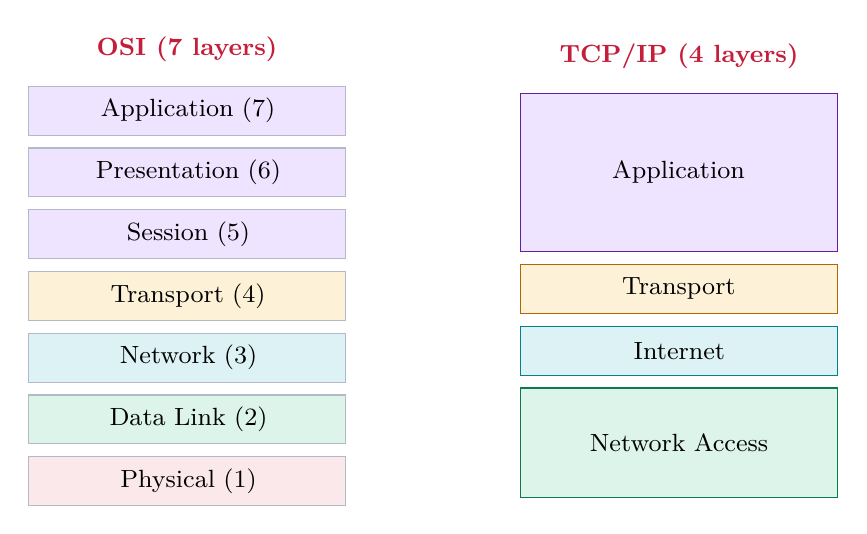
\begin{tikzpicture}[node distance=0.15cm]
  % OSI left column — 7 layers stacked top to bottom
  \node[rectangle, draw=mgframe, fill=hdrpurple, text width=3.8cm, align=center,
        minimum height=0.62cm, font=\small] (L7) {Application (7)};
  \node[rectangle, draw=mgframe, fill=hdrpurple, text width=3.8cm, align=center,
        minimum height=0.62cm, font=\small, below=0.15cm of L7] (L6) {Presentation (6)};
  \node[rectangle, draw=mgframe, fill=hdrpurple, text width=3.8cm, align=center,
        minimum height=0.62cm, font=\small, below=0.15cm of L6] (L5) {Session (5)};
  \node[rectangle, draw=mgframe, fill=hdramber, text width=3.8cm, align=center,
        minimum height=0.62cm, font=\small, below=0.15cm of L5] (L4) {Transport (4)};
  \node[rectangle, draw=mgframe, fill=hdrteal, text width=3.8cm, align=center,
        minimum height=0.62cm, font=\small, below=0.15cm of L4] (L3) {Network (3)};
  \node[rectangle, draw=mgframe, fill=hdrgreen, text width=3.8cm, align=center,
        minimum height=0.62cm, font=\small, below=0.15cm of L3] (L2) {Data Link (2)};
  \node[rectangle, draw=mgframe, fill=hdrred, text width=3.8cm, align=center,
        minimum height=0.62cm, font=\small, below=0.15cm of L2] (L1) {Physical (1)};
  % OSI label
  \node[above=0.18cm of L7, font=\small\bfseries\color{myred}] {OSI (7 layers)};
  % TCP/IP right column — 4 layers
  \node[rectangle, draw=mypurple, fill=hdrpurple, text width=3.8cm, align=center,
        minimum height=2.01cm, font=\small, right=2.2cm of L6] (app) {Application};
  \node[rectangle, draw=myamber, fill=hdramber, text width=3.8cm, align=center,
        minimum height=0.62cm, font=\small, below=0.15cm of app] (trans) {Transport};
  \node[rectangle, draw=myteal, fill=hdrteal, text width=3.8cm, align=center,
        minimum height=0.62cm, font=\small, below=0.15cm of trans] (inet) {Internet};
  \node[rectangle, draw=mygreen, fill=hdrgreen, text width=3.8cm, align=center,
        minimum height=1.39cm, font=\small, below=0.15cm of inet] (netacc) {Network Access};
  % TCP/IP label
  \node[above=0.18cm of app, font=\small\bfseries\color{myred}] {TCP/IP (4 layers)};
\end{tikzpicture}
\end{tcolorbox}

%═══════════════════════════════════════════════════════════════════════════════
\section{Physical Level}
%═══════════════════════════════════════════════════════════════════════════════

\subsection{Analog vs.\ Digital Data and Signals}

\begin{tabularx}{\linewidth}{|B{3.0cm}|X|X|}
\hline
\multicolumn{1}{|>{\centering\arraybackslash}p{3.0cm}|}{\textbf{Aspect}} &
\multicolumn{1}{>{\centering\arraybackslash}X|}{\textbf{\color{myteal}Analog}} &
\multicolumn{1}{>{\centering\arraybackslash}X|}{\textbf{\color{myamber}Digital}} \\
\hline
Data            & Continuous values (e.g.\ voice, temperature) & Discrete values (0 and 1) \\
\hline
Signal          & Continuous waveform (sine wave) & Square wave / pulse train \\
\hline
Noise immunity  & Low --- noise degrades signal & High --- regenerated at repeaters \\
\hline
Bandwidth       & Lower bandwidth needed & Higher bandwidth required \\
\hline
Transmission    & Analog transmission (amplifiers) & Digital transmission (repeaters) \\
\hline
\end{tabularx}

\subsection{Transmission Media}

\begin{tcolorbox}[defbox]
\textbf{Transmission Medium:} The physical path between sender and receiver. Classified as \textbf{guided} (wired) or \textbf{unguided} (wireless).
\end{tcolorbox}

\textbf{Guided Media:}
\begin{itemize}[leftmargin=*, itemsep=3pt]
  \item \textbf{Twisted Pair Cable:} Two insulated copper wires twisted together. Reduces electromagnetic interference. Types: UTP (Unshielded) and STP (Shielded). Used in telephone lines, Ethernet (Cat5e, Cat6).
  \item \textbf{Coaxial Cable:} Central conductor surrounded by insulation, metallic shield, and outer jacket. Higher bandwidth than twisted pair. Used in cable TV, older Ethernet (10Base2, 10Base5).
  \item \textbf{Fibre Optic Cable:} Transmits data as light pulses through glass/plastic core. Extremely high bandwidth, immune to EMI, low attenuation. Used in backbone networks, long-distance links.
\end{itemize}

\textbf{Unguided Media (Wireless):}
\begin{itemize}[leftmargin=*, itemsep=3pt]
  \item \textbf{Radio Waves:} Omnidirectional; penetrate walls. Used in AM/FM radio, Wi-Fi, Bluetooth.
  \item \textbf{Microwaves:} Directional; line-of-sight required. Used in satellite communication, cellular networks.
  \item \textbf{Infrared:} Short range; cannot penetrate walls. Used in TV remotes, IrDA.
\end{itemize}

\subsection{Circuit Switching}

\begin{tcolorbox}[defbox]
\textbf{Circuit Switching:} A dedicated communication path is established between sender and receiver for the entire duration of the session. Resources are reserved end-to-end. Used in traditional telephone networks (PSTN).
\end{tcolorbox}

\textbf{Phases of Circuit Switching:}
\begin{enumerate}[label=\textbf{\arabic*.}, leftmargin=*, itemsep=3pt]
  \item \textbf{Circuit Establishment:} A dedicated path is set up through intermediate switches.
  \item \textbf{Data Transfer:} Data flows continuously along the reserved path.
  \item \textbf{Circuit Disconnect:} Path is released and resources freed after communication ends.
\end{enumerate}

\subsubsection*{Space Division Switch}

\begin{tcolorbox}[formulabox, title={\textbf{Space Division Switching}}]
Each connection uses a \textbf{physically separate path} through the switch matrix. A crosspoint (transistor/relay) is activated at the intersection of input and output lines.\\[4pt]
\textbf{Crosspoint matrix:} For $n$ inputs and $n$ outputs, requires $n^2$ crosspoints.\\
\textbf{Advantage:} Simple, simultaneous connections. \textbf{Disadvantage:} Expensive for large $n$.
\end{tcolorbox}

\subsubsection*{Time Division Switch (TDM Bus)}

\begin{tcolorbox}[formulabox, title={\textbf{Time Division Switching}}]
All connections share the \textbf{same physical medium} but are separated in \textbf{time slots}. A Time Slot Interchange (TSI) unit reads input slots and writes them to output slots.\\[4pt]
\textbf{TDM Bus:} A high-speed shared bus; each input is assigned a time slot. The TSI reorders slots to route data to correct outputs.\\
\textbf{Advantage:} Efficient use of medium. \textbf{Disadvantage:} Requires synchronisation.
\end{tcolorbox}

\subsection{Telephone Network}

The Public Switched Telephone Network (PSTN) uses circuit switching. It consists of:
\begin{itemize}[leftmargin=*, itemsep=3pt]
  \item \textbf{Local loops:} Twisted pair from subscriber to local exchange (last mile).
  \item \textbf{Trunks:} High-capacity links (fibre/microwave) between exchanges.
  \item \textbf{Switching offices:} Local, tandem, and toll offices that route calls.
\end{itemize}

\begin{tcolorbox}[tikzbox, title={Telephone Network Structure}]
\centering
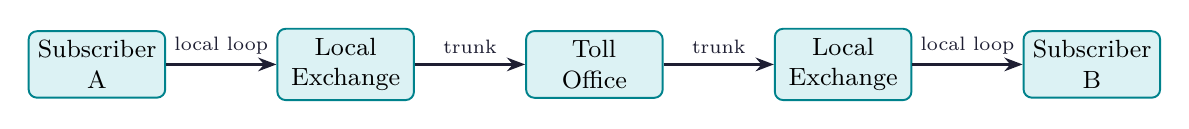
\begin{tikzpicture}[node distance=0.5cm and 1.4cm]
  \node[netnode] (sub1) {Subscriber\\A};
  \node[netnode, right=1.4cm of sub1] (local1) {Local\\Exchange};
  \node[netnode, right=1.4cm of local1] (toll) {Toll\\Office};
  \node[netnode, right=1.4cm of toll] (local2) {Local\\Exchange};
  \node[netnode, right=1.4cm of local2] (sub2) {Subscriber\\B};
  \draw[arrow] (sub1) -- node[above]{\scriptsize local loop} (local1);
  \draw[arrow] (local1) -- node[above]{\scriptsize trunk} (toll);
  \draw[arrow] (toll) -- node[above]{\scriptsize trunk} (local2);
  \draw[arrow] (local2) -- node[above]{\scriptsize local loop} (sub2);
\end{tikzpicture}
\end{tcolorbox}

%═══════════════════════════════════════════════════════════════════════════════
\section{Multiplexing: FDM, TDM, and WDM}
%═══════════════════════════════════════════════════════════════════════════════

\begin{tcolorbox}[defbox]
\textbf{Multiplexing:} A technique that allows multiple signals to share a single transmission medium simultaneously. A \textbf{multiplexer (MUX)} combines signals at the sender; a \textbf{demultiplexer (DEMUX)} separates them at the receiver.
\end{tcolorbox}

\begin{tcolorbox}[tikzbox, title={General Multiplexing Concept}]
\centering
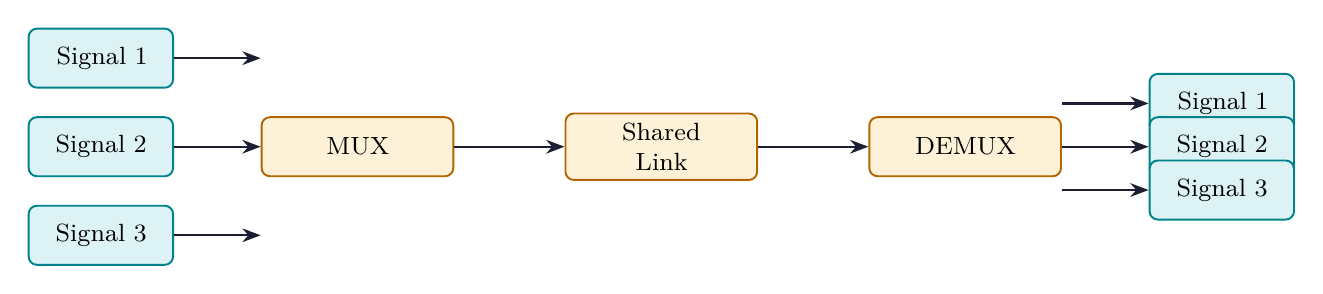
\begin{tikzpicture}[node distance=0.3cm and 0.9cm,
  sblock/.style={rectangle, draw=myteal, fill=hdrteal, text width=1.6cm,
    align=center, minimum height=0.75cm, font=\small, rounded corners=3pt, line width=0.7pt},
  chan/.style={rectangle, draw=myamber, fill=hdramber, text width=2.2cm,
    align=center, minimum height=0.75cm, font=\small, rounded corners=3pt, line width=0.7pt}]
  % Input signals
  \node[sblock] (s1) {Signal 1};
  \node[sblock, below=0.35cm of s1] (s2) {Signal 2};
  \node[sblock, below=0.35cm of s2] (s3) {Signal 3};
  % MUX
  \node[chan, right=1.1cm of s2] (mux) {MUX};
  % Shared link
  \node[chan, right=1.4cm of mux] (link) {Shared\\Link};
  % DEMUX
  \node[chan, right=1.4cm of link] (demux) {DEMUX};
  % Output signals
  \node[sblock, right=1.1cm of demux, yshift=0.55cm] (r1) {Signal 1};
  \node[sblock, right=1.1cm of demux] (r2) {Signal 2};
  \node[sblock, right=1.1cm of demux, yshift=-0.55cm] (r3) {Signal 3};
  % Arrows in
  \draw[arrow] (s1.east) -- (mux.west |- s1.east);
  \draw[arrow] (s2.east) -- (mux.west);
  \draw[arrow] (s3.east) -- (mux.west |- s3.east);
  % MUX to link to DEMUX
  \draw[arrow] (mux) -- (link);
  \draw[arrow] (link) -- (demux);
  % Arrows out
  \draw[arrow] (demux.east |- r1.west) -- (r1.west);
  \draw[arrow] (demux.east) -- (r2.west);
  \draw[arrow] (demux.east |- r3.west) -- (r3.west);
\end{tikzpicture}
\end{tcolorbox}

%───────────────────────────────────────────────────────────────────────────────
\subsection{Frequency Division Multiplexing (FDM)}
%───────────────────────────────────────────────────────────────────────────────

\begin{tcolorbox}[defbox]
\textbf{FDM (Frequency Division Multiplexing):} The total bandwidth of the medium is divided into non-overlapping \textbf{frequency bands (sub-channels)}. Each signal is modulated onto a different carrier frequency and transmitted simultaneously. Used for \textbf{analog signals}.
\end{tcolorbox}

\textbf{Working:}
\begin{enumerate}[label=\textbf{\arabic*.}, leftmargin=*, itemsep=3pt]
  \item Each input signal is modulated onto a unique carrier frequency $f_1, f_2, \ldots, f_n$.
  \item Guard bands (unused frequency gaps) separate adjacent channels to prevent interference.
  \item All modulated signals are combined and transmitted over the shared medium.
  \item At the receiver, bandpass filters separate each channel; demodulation recovers the original signal.
\end{enumerate}

\begin{tcolorbox}[formulabox, title={\textbf{FDM Key Formulas}}]
\begin{tabularx}{\linewidth}{B{4.5cm} X}
Channel bandwidth    & $B_{ch} = f_{upper} - f_{lower}$ \\[4pt]
Total bandwidth      & $B_{total} = n \times B_{ch} + (n-1) \times B_{guard}$ \\[4pt]
Guard band           & Unused frequency gap between adjacent channels to prevent inter-channel interference \\[4pt]
Carrier frequencies  & $f_1 < f_2 < \cdots < f_n$, each separated by at least $B_{ch} + B_{guard}$
\end{tabularx}
\end{tcolorbox}

\begin{tcolorbox}[tikzbox, title={FDM --- Frequency Spectrum Allocation}]
\centering
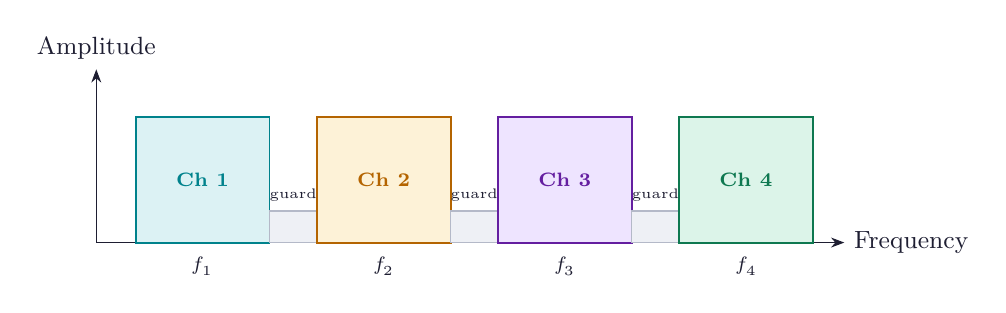
\begin{tikzpicture}[scale=1.0]
  % Frequency axis
  \draw[-Stealth, thin, color=mydark] (0,0) -- (9.5,0) node[right, font=\small] {Frequency};
  \draw[-Stealth, thin, color=mydark] (0,0) -- (0,2.2) node[above, font=\small] {Amplitude};
  % Channel 1
  \fill[hdrteal, draw=myteal, line width=0.7pt] (0.5,0) rectangle (2.2,1.6);
  \node[font=\scriptsize\bfseries, color=myteal] at (1.35,0.8) {Ch 1};
  \node[font=\scriptsize, color=mydark] at (1.35,-0.3) {$f_1$};
  % Guard band 1
  \fill[hdrgray, draw=mgframe, line width=0.5pt] (2.2,0) rectangle (2.8,0.4);
  \node[font=\tiny, color=mydark] at (2.5,0.6) {guard};
  % Channel 2
  \fill[hdramber, draw=myamber, line width=0.7pt] (2.8,0) rectangle (4.5,1.6);
  \node[font=\scriptsize\bfseries, color=myamber] at (3.65,0.8) {Ch 2};
  \node[font=\scriptsize, color=mydark] at (3.65,-0.3) {$f_2$};
  % Guard band 2
  \fill[hdrgray, draw=mgframe, line width=0.5pt] (4.5,0) rectangle (5.1,0.4);
  \node[font=\tiny, color=mydark] at (4.8,0.6) {guard};
  % Channel 3
  \fill[hdrpurple, draw=mypurple, line width=0.7pt] (5.1,0) rectangle (6.8,1.6);
  \node[font=\scriptsize\bfseries, color=mypurple] at (5.95,0.8) {Ch 3};
  \node[font=\scriptsize, color=mydark] at (5.95,-0.3) {$f_3$};
  % Guard band 3
  \fill[hdrgray, draw=mgframe, line width=0.5pt] (6.8,0) rectangle (7.4,0.4);
  \node[font=\tiny, color=mydark] at (7.1,0.6) {guard};
  % Channel 4
  \fill[hdrgreen, draw=mygreen, line width=0.7pt] (7.4,0) rectangle (9.1,1.6);
  \node[font=\scriptsize\bfseries, color=mygreen] at (8.25,0.8) {Ch 4};
  \node[font=\scriptsize, color=mydark] at (8.25,-0.3) {$f_4$};
\end{tikzpicture}
\end{tcolorbox}

\begin{tabularx}{\linewidth}{|B{3.2cm}|X|}
\hline
\multicolumn{1}{|>{\centering\arraybackslash}p{3.2cm}|}{\textbf{\color{myteal}Aspect}} &
\multicolumn{1}{>{\centering\arraybackslash}X|}{\textbf{\color{myteal}Details}} \\
\hline
Signal type       & Analog signals \\
\hline
Separation method & Different carrier frequencies; guard bands prevent overlap \\
\hline
Simultaneous?     & Yes --- all channels transmit at the same time \\
\hline
Applications      & AM/FM radio, cable TV, ADSL, first-generation cellular (1G) \\
\hline
Advantage         & Simple; no synchronisation needed; all channels always active \\
\hline
Disadvantage      & Guard bands waste bandwidth; susceptible to intermodulation noise \\
\hline
\end{tabularx}

%───────────────────────────────────────────────────────────────────────────────
\subsection{Time Division Multiplexing (TDM)}
%───────────────────────────────────────────────────────────────────────────────

\begin{tcolorbox}[defbox]
\textbf{TDM (Time Division Multiplexing):} The time on the shared channel is divided into fixed \textbf{time slots}. Each input signal is assigned a slot in a repeating \textbf{frame}. Used for \textbf{digital signals}.
\end{tcolorbox}

\textbf{Two types of TDM:}

\begin{tcolorbox}[formulabox, title={\textbf{Synchronous TDM}}]
Each input is assigned a \textbf{fixed time slot} in every frame, regardless of whether it has data to send. Slots are pre-allocated.\\[4pt]
\begin{tabularx}{\linewidth}{B{4.0cm} X}
Frame duration    & $T_f = n \times T_s$ \quad ($n$ = number of channels, $T_s$ = slot duration) \\[4pt]
Output bit rate   & $R_{out} = n \times R_{in}$ \quad (output must be $n$ times faster than each input) \\[4pt]
Frame efficiency  & Can be low --- empty slots wasted if a channel has no data
\end{tabularx}
\end{tcolorbox}

\begin{tcolorbox}[formulabox, title={\textbf{Statistical (Asynchronous) TDM}}]
Slots are allocated \textbf{dynamically} --- only to channels that have data. Each slot carries an \textbf{address header} to identify the source.\\[4pt]
\begin{tabularx}{\linewidth}{B{4.0cm} X}
Efficiency        & Higher than synchronous TDM; no wasted slots \\[4pt]
Overhead          & Address field added to each slot increases overhead \\[4pt]
Output bit rate   & Less than $n \times R_{in}$ (statistical multiplexing gain)
\end{tabularx}
\end{tcolorbox}

\begin{tcolorbox}[tikzbox, title={Synchronous TDM --- Frame Structure (4 channels)}]
\centering
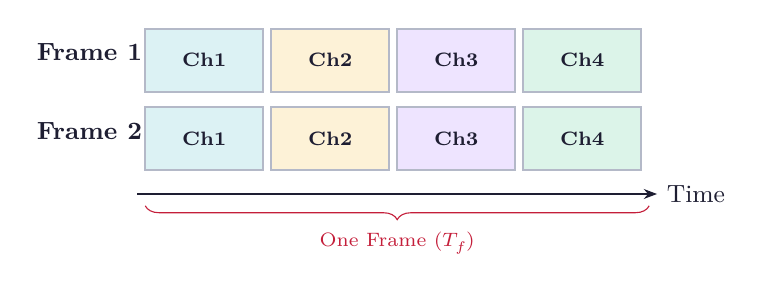
\begin{tikzpicture}[scale=1.0]
  % Frame label
  \node[font=\small\bfseries\color{mydark}, anchor=west] at (0, 1.6) {Frame 1:};
  % 4 slots in frame 1
  \foreach \i/\col/\lbl in {0/hdrteal/Ch1, 1/hdramber/Ch2, 2/hdrpurple/Ch3, 3/hdrgreen/Ch4} {
    \fill[\col, draw=mgframe, line width=0.7pt] ({1.5+\i*1.6}, 1.1) rectangle ({1.5+\i*1.6+1.5}, 1.9);
    \node[font=\scriptsize\bfseries\color{mydark}] at ({1.5+\i*1.6+0.75}, 1.5) {\lbl};
  }
  % Frame 2
  \node[font=\small\bfseries\color{mydark}, anchor=west] at (0, 0.6) {Frame 2:};
  \foreach \i/\col/\lbl in {0/hdrteal/Ch1, 1/hdramber/Ch2, 2/hdrpurple/Ch3, 3/hdrgreen/Ch4} {
    \fill[\col, draw=mgframe, line width=0.7pt] ({1.5+\i*1.6}, 0.1) rectangle ({1.5+\i*1.6+1.5}, 0.9);
    \node[font=\scriptsize\bfseries\color{mydark}] at ({1.5+\i*1.6+0.75}, 0.5) {\lbl};
  }
  % Time arrow
  \draw[-Stealth, thin, color=mydark] (1.4, -0.2) -- (8.0, -0.2) node[right, font=\small] {Time};
  % Brace for one frame
  \draw[decorate, decoration={brace, amplitude=5pt, mirror}, color=myred]
    (1.5, -0.35) -- (7.9, -0.35) node[midway, below=6pt, font=\scriptsize\color{myred}] {One Frame ($T_f$)};
\end{tikzpicture}
\end{tcolorbox}

\begin{tabularx}{\linewidth}{|B{3.2cm}|X|X|}
\hline
\multicolumn{1}{|>{\centering\arraybackslash}p{3.2cm}|}{\textbf{\color{myteal}Aspect}} &
\multicolumn{1}{>{\centering\arraybackslash}X|}{\textbf{\color{myteal}Synchronous TDM}} &
\multicolumn{1}{>{\centering\arraybackslash}X|}{\textbf{\color{myteal}Statistical TDM}} \\
\hline
Slot allocation   & Fixed; pre-assigned per channel & Dynamic; only active channels get slots \\
\hline
Address header    & Not needed (position identifies channel) & Required (slot carries source address) \\
\hline
Efficiency        & Low if channels idle & High; no wasted slots \\
\hline
Output rate       & $n \times R_{in}$ (fixed) & Less than $n \times R_{in}$ \\
\hline
Example           & T1/E1 lines, SONET & ATM, packet-switched networks \\
\hline
\end{tabularx}

%───────────────────────────────────────────────────────────────────────────────
\subsection{Wavelength Division Multiplexing (WDM)}
%───────────────────────────────────────────────────────────────────────────────

\begin{tcolorbox}[defbox]
\textbf{WDM (Wavelength Division Multiplexing):} Multiple optical signals are transmitted simultaneously over a single \textbf{fibre optic cable}, each on a different \textbf{wavelength (colour) of light}. Conceptually identical to FDM but applied to optical frequencies. Used in high-capacity fibre networks.
\end{tcolorbox}

\textbf{Working:}
\begin{enumerate}[label=\textbf{\arabic*.}, leftmargin=*, itemsep=3pt]
  \item Each data stream modulates a laser of a distinct wavelength $\lambda_1, \lambda_2, \ldots, \lambda_n$.
  \item A \textbf{prism or optical multiplexer} combines all wavelengths onto one fibre.
  \item The combined beam travels through the fibre.
  \item At the receiver, a \textbf{prism or optical demultiplexer} separates the wavelengths.
  \item Each wavelength is detected by a photodetector and demodulated.
\end{enumerate}

\begin{tcolorbox}[tikzbox, title={WDM --- Wavelength Multiplexing on Fibre}]
\centering
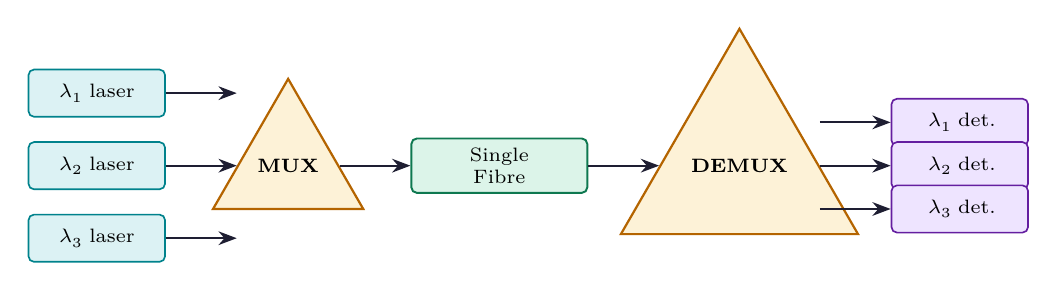
\begin{tikzpicture}[node distance=0.3cm and 0.8cm,
  laser/.style={rectangle, draw=myteal, fill=hdrteal, text width=1.5cm,
    align=center, minimum height=0.6cm, font=\scriptsize, rounded corners=2pt, line width=0.6pt},
  prism/.style={regular polygon, regular polygon sides=3, draw=myamber, fill=hdramber,
    minimum size=1.1cm, font=\scriptsize\bfseries, inner sep=0pt, line width=0.8pt},
  fibre/.style={rectangle, draw=mygreen, fill=hdrgreen, text width=2.0cm,
    align=center, minimum height=0.6cm, font=\scriptsize, rounded corners=2pt, line width=0.7pt},
  det/.style={rectangle, draw=mypurple, fill=hdrpurple, text width=1.5cm,
    align=center, minimum height=0.6cm, font=\scriptsize, rounded corners=2pt, line width=0.6pt}]
  % Lasers
  \node[laser] (l1) {$\lambda_1$ laser};
  \node[laser, below=0.3cm of l1] (l2) {$\lambda_2$ laser};
  \node[laser, below=0.3cm of l2] (l3) {$\lambda_3$ laser};
  % MUX prism
  \node[prism, right=0.9cm of l2] (mux) {MUX};
  % Fibre
  \node[fibre, right=0.9cm of mux] (fibre) {Single\\Fibre};
  % DEMUX prism
  \node[prism, right=0.9cm of fibre] (demux) {DEMUX};
  % Detectors
  \node[det, right=0.9cm of demux, yshift=0.55cm] (d1) {$\lambda_1$ det.};
  \node[det, right=0.9cm of demux] (d2) {$\lambda_2$ det.};
  \node[det, right=0.9cm of demux, yshift=-0.55cm] (d3) {$\lambda_3$ det.};
  % Arrows
  \draw[arrow] (l1.east) -- (mux.west |- l1.east);
  \draw[arrow] (l2.east) -- (mux.west);
  \draw[arrow] (l3.east) -- (mux.west |- l3.east);
  \draw[arrow] (mux.east) -- (fibre.west);
  \draw[arrow] (fibre.east) -- (demux.west);
  \draw[arrow] (demux.east |- d1.west) -- (d1.west);
  \draw[arrow] (demux.east) -- (d2.west);
  \draw[arrow] (demux.east |- d3.west) -- (d3.west);
\end{tikzpicture}
\end{tcolorbox}

\textbf{Types of WDM:}
\begin{itemize}[leftmargin=*, itemsep=3pt]
  \item \textbf{CWDM (Coarse WDM):} Fewer channels (up to 18), wider wavelength spacing (20 nm). Lower cost, shorter distances.
  \item \textbf{DWDM (Dense WDM):} Many channels (40--160+), very narrow spacing (0.8 nm or less). Used in long-haul backbone networks. Capacity up to several Tbps on one fibre.
\end{itemize}

\begin{tabularx}{\linewidth}{|B{3.2cm}|X|}
\hline
\multicolumn{1}{|>{\centering\arraybackslash}p{3.2cm}|}{\textbf{\color{myteal}Aspect}} &
\multicolumn{1}{>{\centering\arraybackslash}X|}{\textbf{\color{myteal}Details}} \\
\hline
Medium            & Fibre optic cable only \\
\hline
Separation method & Different wavelengths (colours) of light \\
\hline
Analogy           & FDM applied to optical domain \\
\hline
Capacity          & DWDM: 40--160+ channels; Tbps aggregate \\
\hline
Applications      & Internet backbone, long-haul telecom, submarine cables \\
\hline
Advantage         & Enormous capacity; each wavelength is independent \\
\hline
Disadvantage      & Expensive equipment; requires precise laser wavelengths \\
\hline
\end{tabularx}

%───────────────────────────────────────────────────────────────────────────────
\subsection{FDM vs.\ TDM vs.\ WDM --- Comparison}
%───────────────────────────────────────────────────────────────────────────────

\par\noindent
\begin{tabularx}{\linewidth}{|B{3.0cm}|>{\small\raggedright\arraybackslash}X|>{\small\raggedright\arraybackslash}X|>{\small\raggedright\arraybackslash}X|}
\hline
\multicolumn{1}{|>{\centering\arraybackslash}p{3.0cm}|}{\textbf{Parameter}} &
\multicolumn{1}{>{\centering\arraybackslash}X|}{\textbf{\color{myteal}FDM}} &
\multicolumn{1}{>{\centering\arraybackslash}X|}{\textbf{\color{myamber}TDM}} &
\multicolumn{1}{>{\centering\arraybackslash}X|}{\textbf{\color{mygreen}WDM}} \\
\hline
Full form         & Frequency Division Multiplexing & Time Division Multiplexing & Wavelength Division Multiplexing \\
\hline
Signal type       & Analog & Digital & Optical (light) \\
\hline
Sharing basis     & Frequency bands & Time slots & Wavelengths of light \\
\hline
Medium            & Coaxial, twisted pair, air & Any digital medium & Fibre optic only \\
\hline
Synchronisation   & Not required & Required (sync TDM) & Not required \\
\hline
Guard bands       & Required & Not needed & Not needed (wavelength spacing) \\
\hline
Applications      & Radio, cable TV, ADSL & T1/E1, SONET, GSM & Internet backbone, DWDM \\
\hline
Capacity          & Moderate & High & Very high (Tbps) \\
\hline
\end{tabularx}

%═══════════════════════════════════════════════════════════════════════════════
% QUICK REVISION PAGE
%═══════════════════════════════════════════════════════════════════════════════
\newpage
\begin{center}
  {\large\bfseries\color{myred} Quick Revision --- Module 1}\\[3pt]
  {\small\color{mydark} Data Communication, Networking Overview \& Physical Level $|$ EC602}
\end{center}
\noindent{\color{myred}\rule{\linewidth}{1.2pt}}
\vspace{4pt}

\begin{tcolorbox}[formulabox, title={\textbf{Key Facts at a Glance}}]
\begin{tabularx}{\linewidth}{B{4.8cm} X}
OSI Layers (top to bottom) & Application, Presentation, Session, Transport, Network, Data Link, Physical \\[2pt]
TCP/IP Layers              & Application, Transport, Internet, Network Access \\[2pt]
LAN coverage               & Up to a few km (building/campus) \\[2pt]
MAN coverage               & City-wide (5--50 km) \\[2pt]
WAN coverage               & Country / global \\[2pt]
Simplex                    & One direction only \\[2pt]
Half Duplex                & Both directions, not simultaneously \\[2pt]
Full Duplex                & Both directions simultaneously \\[2pt]
Circuit switching phases   & Establish $\to$ Transfer $\to$ Disconnect \\[2pt]
Space division crosspoints & $n^2$ for $n \times n$ \\[2pt]
TDM output bit rate        & $R_{out} = n \times R_{in}$ (synchronous TDM) \\[2pt]
TDM frame duration         & $T_f = n \times T_s$ \\[2pt]
FDM total bandwidth        & $B_{total} = n \times B_{ch} + (n-1) \times B_{guard}$ \\[2pt]
WDM                        & FDM applied to optical domain; uses wavelengths of light switch \\[2pt]
ASCII                      & 7-bit encoding, 128 characters \\[2pt]
Unicode                    & 32-bit encoding, universal character set \\[2pt]
\end{tabularx}
\end{tcolorbox}

\vspace{6pt}

\begin{tcolorbox}[defbox, title={\textbf{One-Line Definitions}}]
\begin{itemize}[leftmargin=*, itemsep=3pt, topsep=0pt]
  \item \textbf{Protocol:} Set of rules governing communication between devices.
  \item \textbf{Topology:} Geometric arrangement of devices and links in a network.
  \item \textbf{LAN:} Local Area Network; high-speed network within a building or campus.
  \item \textbf{WAN:} Wide Area Network; spans cities, countries, or the globe.
  \item \textbf{OSI Model:} 7-layer ISO standard for network communication.
  \item \textbf{TCP/IP Model:} 4-layer practical model underlying the Internet.
  \item \textbf{Circuit Switching:} Dedicated path reserved for entire session duration.
  \item \textbf{TDM:} Time Division Multiplexing; shares medium by assigning time slots to each channel.
  \item \textbf{FDM:} Frequency Division Multiplexing; divides bandwidth into frequency bands for analog signals.
  \item \textbf{WDM:} Wavelength Division Multiplexing; uses different light wavelengths on a single fibre optic cable.
  \item \textbf{Statistical TDM:} Dynamic slot allocation; only active channels get slots, improving efficiency.
  \item \textbf{DWDM:} Dense WDM; 40--160+ channels with narrow wavelength spacing; used in backbone networks.
  \item \textbf{Guided Media:} Physical wired medium (twisted pair, coaxial, fibre optic).
  \item \textbf{Unguided Media:} Wireless medium (radio, microwave, infrared).
  \item \textbf{Full Duplex:} Simultaneous two-way communication.
  \item \textbf{ASCII:} American Standard Code for Information Interchange; 7-bit text encoding.
\end{itemize}
\end{tcolorbox}

\vspace{6pt}

\begin{tcolorbox}[exambox, title={\textbf{Frequently Asked / Viva Questions}}]
\begin{enumerate}[leftmargin=*, topsep=0pt, label=\textbf{Q\arabic*.}, itemsep=8pt]
  \item \Q{What are the five components of data communication?} Sender, Receiver, Message, Medium, and Protocol.
  \item \Q{Difference between simplex, half duplex, and full duplex?} Simplex: one direction only. Half duplex: both directions but not simultaneously. Full duplex: both directions simultaneously.
  \item \Q{How many layers does the OSI model have? Name them.} 7 layers: Physical, Data Link, Network, Transport, Session, Presentation, Application (bottom to top).
  \item \Q{What is the PDU at the Network layer?} Packet.
  \item \Q{What is the PDU at the Data Link layer?} Frame.
  \item \Q{How does TCP/IP differ from OSI?} TCP/IP has 4 layers vs.\ OSI's 7; TCP/IP is practical and protocol-specific; OSI is a conceptual reference model.
  \item \Q{What is circuit switching?} A dedicated communication path is established and reserved for the entire session. Used in PSTN.
  \item \Q{What is the difference between space division and time division switching?} Space division uses separate physical paths (crosspoint matrix); time division shares one medium using time slots (TSI).
  \item \Q{What is the advantage of fibre optic over copper?} Higher bandwidth, lower attenuation, immune to EMI, more secure.
  \item \Q{What is a MAN?} Metropolitan Area Network; covers a city (5--50 km); e.g.\ cable TV network, WiMAX.
  \item \Q{What does ASCII stand for?} American Standard Code for Information Interchange; 7-bit encoding for 128 characters.
  \item \Q{Why is full duplex preferred over half duplex?} Full duplex allows simultaneous two-way communication, doubling effective throughput compared to half duplex.
  \item \Q{What is multiplexing and why is it used?} Multiplexing allows multiple signals to share a single transmission medium, reducing cost and making efficient use of bandwidth.
  \item \Q{What is the difference between FDM and TDM?} FDM divides the bandwidth into frequency bands for analog signals; TDM divides time into slots for digital signals. FDM channels transmit simultaneously; TDM channels take turns.
  \item \Q{What is WDM and where is it used?} WDM transmits multiple optical signals on one fibre using different wavelengths of light. Used in Internet backbone and long-haul telecom (DWDM supports 40--160+ channels).
  \item \Q{What is the difference between synchronous and statistical TDM?} Synchronous TDM assigns fixed slots to each channel regardless of activity (wastes slots if idle). Statistical TDM allocates slots dynamically only to active channels, improving efficiency but requiring address headers.
\end{enumerate}
\end{tcolorbox}

\vspace{6pt}

\begin{tcolorbox}[tikzbox, title={\textbf{OSI Layer Summary Table}}]
\begin{tabularx}{\linewidth}{|>{\centering\arraybackslash}p{0.5cm}|B{2.8cm}|X|>{\centering\arraybackslash}p{2.2cm}|}
\hline
\textbf{\#} & \textbf{Layer} & \textbf{Key Function} & \textbf{PDU} \\
\hline
7 & Application  & User-facing services (HTTP, FTP, DNS) & Data \\
\hline
6 & Presentation & Encryption, compression, translation & Data \\
\hline
5 & Session      & Session management, synchronisation & Data \\
\hline
4 & Transport    & End-to-end delivery, TCP/UDP & Segment \\
\hline
3 & Network      & Routing, IP addressing & Packet \\
\hline
2 & Data Link    & Framing, MAC, error detection & Frame \\
\hline
1 & Physical     & Bit transmission over medium & Bits \\
\hline
\end{tabularx}
\end{tcolorbox}


% -- Module 2 -----------------------------------------------------------------
\modulestart{2}{Data Link Layer}

\section{Data Link Layer}
%═══════════════════════════════════════════════════════════════════════════════

\begin{tcolorbox}[defbox]
\textbf{Data Link Layer (Layer 2):} Responsible for \textit{node-to-node} delivery of frames. It handles framing, physical addressing (MAC), error detection/correction, and flow control between adjacent nodes.
\end{tcolorbox}

\subsection{Types of Errors}

\begin{tabularx}{\linewidth}{|B{3.0cm}|X|}
\hline
\multicolumn{1}{|>{\centering\arraybackslash}p{3.0cm}|}{\textbf{\color{mygreen}Error Type}} &
\multicolumn{1}{>{\centering\arraybackslash}X|}{\textbf{\color{mygreen}Description}} \\
\hline
Single-bit error   & Only one bit in the data unit is changed (0 to 1 or 1 to 0). Rare in serial transmission. \\
\hline
Burst error        & Two or more consecutive bits are corrupted. More common; caused by noise bursts. Length = from first to last corrupted bit. \\
\hline
\end{tabularx}

\subsection{Framing}

\begin{tcolorbox}[defbox]
\textbf{Framing:} The process of dividing a stream of bits from the network layer into manageable data units called \textbf{frames}. Allows the receiver to identify the start and end of each frame.
\end{tcolorbox}

\subsubsection*{Character (Byte) Stuffing}
Used when frames contain text data. A special \textbf{flag byte} (e.g.\ \texttt{FLAG}) marks frame boundaries. If the flag byte appears in the data, an \textbf{escape byte (ESC)} is inserted before it.
\begin{itemize}[leftmargin=*, itemsep=2pt]
  \item If data contains \texttt{FLAG}: insert \texttt{ESC} before it.
  \item If data contains \texttt{ESC}: insert another \texttt{ESC} before it.
  \item Receiver removes the stuffed \texttt{ESC} bytes.
\end{itemize}

\subsubsection*{Bit Stuffing}
Used in bit-oriented protocols (e.g.\ HDLC). Flag pattern is \texttt{01111110}. To prevent this pattern from appearing in data:
\begin{itemize}[leftmargin=*, itemsep=2pt]
  \item \textbf{Sender:} After every 5 consecutive 1s in data, insert a 0.
  \item \textbf{Receiver:} After every 5 consecutive 1s, if next bit is 0, remove it; if 1, it is a flag.
\end{itemize}

\subsection{Error Detection and Correction}

\subsubsection*{Parity Check}
\begin{tcolorbox}[formulabox, title={\textbf{Parity Check}}]
A single parity bit is appended to make the total number of 1s \textbf{even} (even parity) or \textbf{odd} (odd parity).\\
\textbf{Limitation:} Detects only \textit{odd} number of bit errors; cannot detect even-number errors or correct errors.
\end{tcolorbox}

\subsubsection*{Cyclic Redundancy Check (CRC)}
\begin{tcolorbox}[formulabox, title={\textbf{CRC --- Most Widely Used Error Detection}}]
\textbf{Concept:} Treat the data as a binary polynomial. Divide by a \textbf{generator polynomial} $G(x)$. Append the remainder (CRC bits) to the data.\\[4pt]
\textbf{Sender:}
\begin{enumerate}[label=\arabic*., leftmargin=*, itemsep=2pt, topsep=0pt]
  \item Append $r$ zeros to data ($r$ = degree of $G(x)$).
  \item Divide augmented data by $G(x)$ using modulo-2 division (XOR).
  \item Replace appended zeros with remainder $R(x)$ --- this is the CRC.
\end{enumerate}
\textbf{Receiver:} Divide received frame by $G(x)$. If remainder $= 0$, no error; else error detected.\\[4pt]
\textbf{Common generators:} CRC-8 ($x^8+x^2+x+1$), CRC-16, CRC-32 (Ethernet).
\end{tcolorbox}

\subsubsection*{Hamming Code (Error Correction)}
\begin{tcolorbox}[formulabox, title={\textbf{Hamming Code}}]
Adds \textbf{redundant parity bits} at positions that are powers of 2 ($p_1, p_2, p_4, p_8, \ldots$). Each parity bit covers specific data bits.\\[4pt]
\textbf{Minimum redundant bits:} For $m$ data bits, need $r$ parity bits such that $2^r \geq m + r + 1$.\\[4pt]
\textbf{Error correction:} Receiver recalculates parity bits; the binary value of failing parity positions gives the \textbf{error position} (syndrome). Flip that bit to correct.\\
\textbf{Capability:} Detects and corrects \textbf{single-bit errors}; detects (not corrects) double-bit errors.
\end{tcolorbox}

\subsection{Flow Control}

\begin{tcolorbox}[defbox]
\textbf{Flow Control:} Mechanism to prevent a fast sender from overwhelming a slow receiver. The receiver controls the rate at which the sender transmits data.
\end{tcolorbox}

\begin{tabularx}{\linewidth}{|B{3.0cm}|X|}
\hline
\multicolumn{1}{|>{\centering\arraybackslash}p{3.0cm}|}{\textbf{\color{myteal}Method}} &
\multicolumn{1}{>{\centering\arraybackslash}X|}{\textbf{\color{myteal}Description}} \\
\hline
Stop-and-Wait      & Sender sends one frame, waits for ACK before sending next. Simple but inefficient (low throughput). \\
\hline
Sliding Window     & Sender can transmit multiple frames (window size $W$) before needing ACK. Improves efficiency. \\
\hline
\end{tabularx}

\subsection{ARQ Protocols (Automatic Repeat reQuest)}

\begin{tcolorbox}[defbox]
\textbf{ARQ:} Error control mechanism combining error detection with retransmission. Uses ACK (acknowledgement) and NAK (negative acknowledgement) to ensure reliable delivery.
\end{tcolorbox}

\subsubsection*{Stop-and-Wait ARQ}
\begin{tcolorbox}[formulabox, title={\textbf{Stop-and-Wait ARQ}}]
Sender transmits one frame and starts a timer. Waits for ACK.\\
\textbf{If ACK received:} Send next frame.\\
\textbf{If NAK or timeout:} Retransmit the same frame.\\[4pt]
\textbf{Efficiency:} $\eta = \dfrac{1}{1 + 2a}$ where $a = \dfrac{T_p}{T_f}$ (propagation delay / frame transmission time).\\
\textbf{Drawback:} Very low efficiency for large $a$ (long links or short frames).
\end{tcolorbox}

\begin{tcolorbox}[tikzbox, title={Stop-and-Wait ARQ --- Message Flow}]
\centering
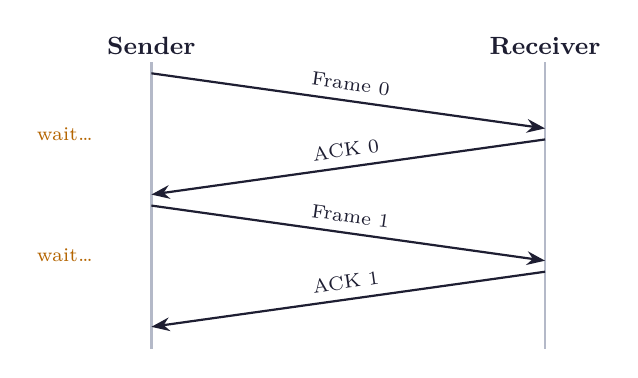
\begin{tikzpicture}[x=1cm, y=0.7cm,
  lbl/.style={font=\small\bfseries\color{mydark}}]
\node[lbl] at (0,5.5) {Sender};
\node[lbl] at (5,5.5) {Receiver};
\draw[thick,color=mgframe] (0,5.2) -- (0,0);
\draw[thick,color=mgframe] (5,5.2) -- (5,0);
% Frame 0
\draw[arrow] (0,5.0) -- node[above,sloped]{\scriptsize Frame 0} (5,4.0);
\draw[arrow] (5,3.8) -- node[above,sloped]{\scriptsize ACK 0} (0,2.8);
% Frame 1
\draw[arrow] (0,2.6) -- node[above,sloped]{\scriptsize Frame 1} (5,1.6);
\draw[arrow] (5,1.4) -- node[above,sloped]{\scriptsize ACK 1} (0,0.4);
% wait annotations
\node[font=\scriptsize\color{myamber}] at (-1.1,3.9) {wait\ldots};
\node[font=\scriptsize\color{myamber}] at (-1.1,1.7) {wait\ldots};
\end{tikzpicture}
\end{tcolorbox}

\subsubsection*{Go-Back-N ARQ (GBN)}
\begin{tcolorbox}[formulabox, title={\textbf{Go-Back-N ARQ}}]
Sender window size $W_s = 2^n - 1$ (for $n$-bit sequence numbers). Receiver window $W_r = 1$.\\
\textbf{On error:} Receiver discards the erroneous frame \textbf{and all subsequent frames}. Sender retransmits from the erroneous frame onwards.\\[4pt]
\textbf{Efficiency:} $\eta = \begin{cases} \dfrac{1}{1+2a} & \text{if } W \geq 1+2a \\ \dfrac{W}{1+2a} & \text{if } W < 1+2a \end{cases}$\\[4pt]
\textbf{Drawback:} Wastes bandwidth retransmitting correctly received frames.
\end{tcolorbox}

\subsubsection*{Selective Repeat ARQ (SR)}
\begin{tcolorbox}[formulabox, title={\textbf{Selective Repeat ARQ}}]
Sender window $W_s = 2^{n-1}$. Receiver window $W_r = 2^{n-1}$.\\
\textbf{On error:} Only the \textbf{erroneous frame} is retransmitted. Receiver buffers out-of-order frames.\\[4pt]
\textbf{Efficiency:} $\eta = \begin{cases} 1 & \text{if } W \geq 1+2a \\ \dfrac{W}{1+2a} & \text{if } W < 1+2a \end{cases}$\\[4pt]
\textbf{Advantage:} More efficient than GBN; \textbf{Disadvantage:} Requires larger receiver buffer.
\end{tcolorbox}

\begin{tabularx}{\linewidth}{|B{3.0cm}|X|X|X|}
\hline
\multicolumn{1}{|>{\centering\arraybackslash}p{3.0cm}|}{\textbf{Parameter}} &
\multicolumn{1}{>{\centering\arraybackslash}X|}{\textbf{Stop-and-Wait}} &
\multicolumn{1}{>{\centering\arraybackslash}X|}{\textbf{Go-Back-N}} &
\multicolumn{1}{>{\centering\arraybackslash}X|}{\textbf{Selective Repeat}} \\
\hline
Sender window   & 1             & $2^n - 1$     & $2^{n-1}$ \\
\hline
Receiver window & 1             & 1             & $2^{n-1}$ \\
\hline
On error        & Retransmit 1  & Retransmit from error & Retransmit only error \\
\hline
Efficiency      & Lowest        & Medium        & Highest \\
\hline
Buffer needed   & Minimal       & Small         & Large \\
\hline
\end{tabularx}

\subsection{HDLC (High-level Data Link Control)}

\begin{tcolorbox}[defbox]
\textbf{HDLC:} A bit-oriented, synchronous data link protocol developed by ISO. Uses bit stuffing for framing. Supports point-to-point and multipoint links.
\end{tcolorbox}

\textbf{HDLC Frame Structure:}\par\noindent
\begin{tabularx}{\linewidth}{|>{\centering\arraybackslash}X|>{\centering\arraybackslash}X|>{\centering\arraybackslash}X|>{\centering\arraybackslash}X|>{\centering\arraybackslash}X|}
\hline
\textbf{\color{myteal}Flag} & \textbf{\color{myteal}Address} & \textbf{\color{myteal}Control} & \textbf{\color{myteal}Data} & \textbf{\color{myteal}FCS + Flag} \\
\hline
01111110 & 8 bits & 8 or 16 bits & Variable & 16/32 bits + 01111110 \\
\hline
\end{tabularx}

\textbf{HDLC Frame Types:}
\begin{itemize}[leftmargin=*, itemsep=3pt]
  \item \textbf{I-frame (Information):} Carries user data; also piggybacks ACK.
  \item \textbf{S-frame (Supervisory):} Flow and error control (ACK, NAK, RNR).
  \item \textbf{U-frame (Unnumbered):} Link management (setup, disconnect).
\end{itemize}

%═══════════════════════════════════════════════════════════════════════════════
\section{Medium Access Sub-layer}
%═══════════════════════════════════════════════════════════════════════════════

\begin{tcolorbox}[defbox]
\textbf{Medium Access Control (MAC):} Sub-layer of the Data Link layer that controls how devices on a shared medium gain access to transmit. Prevents collisions and manages channel allocation.
\end{tcolorbox}

\subsection{Point-to-Point Protocol (PPP)}

\begin{tcolorbox}[defbox]
\textbf{PPP:} A byte-oriented protocol for direct serial links (e.g.\ dial-up, DSL). Provides framing, authentication, and network layer protocol negotiation.
\end{tcolorbox}

\textbf{PPP Components:}
\begin{itemize}[leftmargin=*, itemsep=3pt]
  \item \textbf{LCP (Link Control Protocol):} Establishes, configures, and tests the data link connection.
  \item \textbf{NCP (Network Control Protocol):} Configures network layer protocols (e.g.\ IPCP for IP). One NCP per network layer protocol.
\end{itemize}

\textbf{PPP Frame:} Flag (01111110) $|$ Address (FF) $|$ Control (03) $|$ Protocol $|$ Data $|$ FCS $|$ Flag

\subsection{Token Ring}

\begin{tcolorbox}[defbox]
\textbf{Token Ring (IEEE 802.4/802.5):} A deterministic MAC protocol where a special bit pattern called a \textbf{token} circulates around a ring. Only the station holding the token can transmit.
\end{tcolorbox}

\textbf{Operation:}
\begin{enumerate}[label=\textbf{\arabic*.}, leftmargin=*, itemsep=3pt]
  \item A free token circulates continuously around the ring.
  \item A station wishing to transmit captures the token, changes it to a \textit{busy token}, and appends its frame.
  \item The frame travels around the ring; the destination copies the data.
  \item The originating station removes the frame and releases a new free token.
\end{enumerate}
\textbf{Advantage:} Deterministic, no collisions, fair access. \textbf{Disadvantage:} Token loss/corruption disrupts network.

\begin{tcolorbox}[tikzbox, title={Token Ring Operation}]
\centering
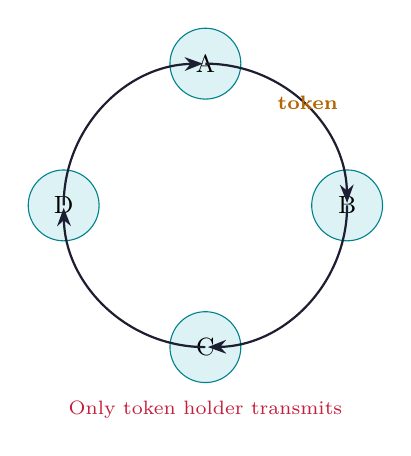
\begin{tikzpicture}[
  sta/.style={circle, draw=myteal, fill=hdrteal, minimum size=0.9cm, font=\small, align=center},
  tok/.style={font=\scriptsize\bfseries\color{myamber}}
]
\foreach \i/\lbl in {0/A, 1/B, 2/C, 3/D} {
  \pgfmathsetmacro\ang{90 - \i*90}
  \node[sta] (S\i) at (\ang:1.8cm) {\lbl};
}
\draw[arrow] (S0) arc[start angle=90, end angle=1, radius=1.8cm];
\draw[arrow] (S1) arc[start angle=0, end angle=-89, radius=1.8cm];
\draw[arrow] (S2) arc[start angle=270, end angle=181, radius=1.8cm];
\draw[arrow] (S3) arc[start angle=180, end angle=91, radius=1.8cm];
\node[tok] at (1.3,1.3) {token};
\node[font=\scriptsize\color{myred}, align=center] at (0,-2.6) {Only token holder transmits};
\end{tikzpicture}
\end{tcolorbox}

\subsection{Multiple Access Protocols}

\subsubsection*{Pure ALOHA}
\begin{tcolorbox}[formulabox, title={\textbf{Pure ALOHA}}]
Stations transmit whenever they have data. If collision occurs, wait a \textbf{random backoff time} and retransmit.\\[4pt]
\textbf{Throughput:} $S = G \cdot e^{-2G}$, maximum $S_{max} = \dfrac{1}{2e} \approx 18.4\%$ at $G = 0.5$.\\
\textbf{Vulnerable period:} $2T_f$ (two frame times).
\end{tcolorbox}

\subsubsection*{Slotted ALOHA}
\begin{tcolorbox}[formulabox, title={\textbf{Slotted ALOHA}}]
Time is divided into slots of size $T_f$. Stations can only transmit at the \textbf{beginning of a slot}.\\[4pt]
\textbf{Throughput:} $S = G \cdot e^{-G}$, maximum $S_{max} = \dfrac{1}{e} \approx 36.8\%$ at $G = 1$.\\
\textbf{Vulnerable period:} $T_f$ (one frame time) --- half that of Pure ALOHA.
\end{tcolorbox}

\subsubsection*{CSMA (Carrier Sense Multiple Access)}
\begin{tcolorbox}[defbox]
\textbf{CSMA:} Before transmitting, a station \textbf{senses the channel}. If busy, it waits; if idle, it transmits. Reduces (but does not eliminate) collisions due to propagation delay.
\end{tcolorbox}

\textbf{CSMA Variants:}\par\noindent
\begin{tabularx}{\linewidth}{|B{3.0cm}|X|}
\hline
\multicolumn{1}{|>{\centering\arraybackslash}p{3.0cm}|}{\textbf{\color{myteal}Variant}} &
\multicolumn{1}{>{\centering\arraybackslash}X|}{\textbf{\color{myteal}Behaviour on Busy Channel}} \\
\hline
1-persistent       & Wait until idle, then transmit immediately with probability 1. High collision risk. \\
\hline
Non-persistent     & Wait a random time, then sense again. Lower collision risk but higher delay. \\
\hline
p-persistent       & When idle, transmit with probability $p$, defer with probability $1-p$. Compromise. \\
\hline
\end{tabularx}

\subsubsection*{CSMA/CD (Collision Detection) --- Ethernet}
\begin{tcolorbox}[formulabox, title={\textbf{CSMA/CD}}]
Used in wired Ethernet (IEEE 802.3). Station senses channel; if idle, transmits and \textbf{monitors for collision simultaneously}.\\
\textbf{On collision:} Transmit jam signal, stop transmission, wait \textbf{binary exponential backoff} time, retry.\\[4pt]
\textbf{Backoff time:} $t = r \times T_{slot}$ where $r$ is random in $[0, 2^k - 1]$, $k$ = attempt number (max 10).\\
\textbf{Minimum frame size:} $L_{min} = 2 \times T_p \times B$ (to detect collision before frame ends).\\
\textbf{Not used in wireless} (cannot detect collision while transmitting).
\end{tcolorbox}

\begin{tcolorbox}[tikzbox, title={CSMA/CD Flowchart}]
\centering
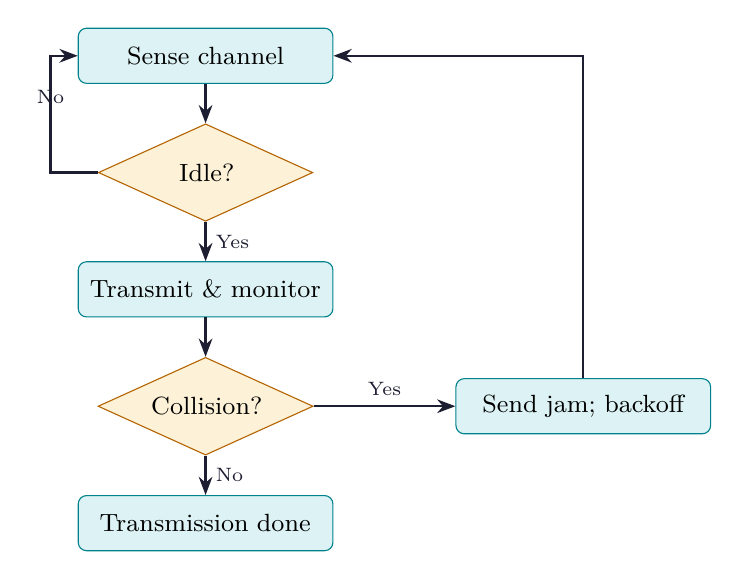
\begin{tikzpicture}[
  proc/.style={rectangle, draw=myteal, fill=hdrteal, text width=3.0cm, align=center, minimum height=0.7cm, font=\small, rounded corners=3pt},
  dec/.style={diamond, draw=myamber, fill=hdramber, text width=2.0cm, align=center, font=\small, aspect=2.2, inner sep=1pt},
  arr/.style={-Stealth, thick, color=mydark},
  node distance=0.5cm
]
\node[proc] (sense) {Sense channel};
\node[dec, below=0.5cm of sense] (idle) {Idle?};
\node[proc, below=0.5cm of idle] (tx) {Transmit \& monitor};
\node[dec, below=0.5cm of tx] (coll) {Collision?};
\node[proc, below=0.5cm of coll] (done) {Transmission done};
\node[proc, right=1.8cm of coll] (jam) {Send jam; backoff};

\draw[arr] (sense) -- (idle);
\draw[arr] (idle) -- node[right]{\scriptsize Yes} (tx);
\draw[arr] (idle.west) -- ++(-0.6,0) |- node[above,pos=0.25]{\scriptsize No} (sense.west);
\draw[arr] (tx) -- (coll);
\draw[arr] (coll) -- node[right]{\scriptsize No} (done);
\draw[arr] (coll) -- node[above]{\scriptsize Yes} (jam);
\draw[arr] (jam.north) |- (sense.east);
\end{tikzpicture}
\end{tcolorbox}

\subsubsection*{CSMA/CA (Collision Avoidance) --- Wi-Fi}
\begin{tcolorbox}[formulabox, title={\textbf{CSMA/CA}}]
Used in wireless networks (IEEE 802.11). Collision \textbf{avoidance} instead of detection (cannot detect collision in wireless).\\[4pt]
\textbf{Mechanism:}
\begin{enumerate}[label=\arabic*., leftmargin=*, itemsep=2pt, topsep=0pt]
  \item Sense channel; if idle for DIFS time, transmit.
  \item If busy, wait for channel to be idle, then wait a random \textbf{backoff} time.
  \item Transmit; receiver sends ACK after SIFS time.
  \item Optional: use \textbf{RTS/CTS} (Request to Send / Clear to Send) to reserve channel.
\end{enumerate}
\end{tcolorbox}

\subsection{Traditional and Fast Ethernet}

\begin{tabularx}{\linewidth}{|B{3.0cm}|X|X|}
\hline
\multicolumn{1}{|>{\centering\arraybackslash}p{3.0cm}|}{\textbf{Parameter}} &
\multicolumn{1}{>{\centering\arraybackslash}X|}{\textbf{\color{myteal}Traditional Ethernet (10 Mbps)}} &
\multicolumn{1}{>{\centering\arraybackslash}X|}{\textbf{\color{myamber}Fast Ethernet (100 Mbps)}} \\
\hline
Standard        & IEEE 802.3                    & IEEE 802.3u \\
\hline
Speed           & 10 Mbps                       & 100 Mbps \\
\hline
MAC protocol    & CSMA/CD                       & CSMA/CD \\
\hline
Frame format    & Same as 802.3                 & Same as 802.3 \\
\hline
Media           & Coaxial, UTP, fibre           & UTP Cat5, fibre \\
\hline
Variants        & 10Base2, 10Base5, 10BaseT     & 100BaseTX, 100BaseT4, 100BaseFX \\
\hline
\end{tabularx}

%═══════════════════════════════════════════════════════════════════════════════
% QUICK REVISION PAGE
%═══════════════════════════════════════════════════════════════════════════════
\newpage
\begin{center}
  {\large\bfseries\color{myred} Quick Revision --- Module 2}\\[3pt]
  {\small\color{mydark} Data Link Layer \& Medium Access Sub-layer $|$ EC602}
\end{center}
\noindent{\color{myred}\rule{\linewidth}{1.2pt}}
\vspace{4pt}

\begin{tcolorbox}[formulabox, title={\textbf{Key Formulas at a Glance}}]
\begin{tabularx}{\linewidth}{B{5.0cm} X}
Stop-and-Wait efficiency    & $\eta = \dfrac{1}{1+2a}$, \quad $a = T_p / T_f$ \\[4pt]
GBN efficiency              & $\eta = \dfrac{W}{1+2a}$ if $W < 1+2a$, else $1$ \\[4pt]
SR efficiency               & $\eta = \dfrac{W}{1+2a}$ if $W < 1+2a$, else $1$ \\[4pt]
GBN sender window           & $W_s = 2^n - 1$ \\[2pt]
SR sender/receiver window   & $W_s = W_r = 2^{n-1}$ \\[2pt]
Pure ALOHA max throughput   & $S_{max} = 1/(2e) \approx 18.4\%$ \\[2pt]
Slotted ALOHA max throughput& $S_{max} = 1/e \approx 36.8\%$ \\[2pt]
Hamming redundant bits      & $2^r \geq m + r + 1$ \\[2pt]
\end{tabularx}
\end{tcolorbox}

\vspace{6pt}

\begin{tcolorbox}[defbox, title={\textbf{One-Line Definitions}}]
\begin{itemize}[leftmargin=*, itemsep=3pt, topsep=0pt]
  \item \textbf{Framing:} Dividing bit stream into frames with identifiable start/end boundaries.
  \item \textbf{Bit Stuffing:} Inserting a 0 after five consecutive 1s to prevent flag pattern in data.
  \item \textbf{CRC:} Error detection using polynomial division; remainder appended as check bits.
  \item \textbf{Hamming Code:} Error-correcting code that adds parity bits at power-of-2 positions.
  \item \textbf{ARQ:} Automatic Repeat reQuest; error control using ACK/NAK and retransmission.
  \item \textbf{Go-Back-N:} On error, retransmit erroneous frame and all subsequent frames.
  \item \textbf{Selective Repeat:} On error, retransmit only the erroneous frame.
  \item \textbf{CSMA/CD:} Sense before transmit; detect collision and use backoff (Ethernet).
  \item \textbf{CSMA/CA:} Sense before transmit; avoid collision using backoff and ACK (Wi-Fi).
  \item \textbf{Token Ring:} Only the station holding the token can transmit; deterministic access.
  \item \textbf{PPP:} Point-to-Point Protocol; uses LCP for link setup and NCP for network config.
  \item \textbf{HDLC:} Bit-oriented DLL protocol; uses bit stuffing; I/S/U frame types.
\end{itemize}
\end{tcolorbox}

\vspace{6pt}

\begin{tcolorbox}[exambox, title={\textbf{Frequently Asked / Viva Questions}}]
\begin{enumerate}[leftmargin=*, topsep=0pt, label=\textbf{Q\arabic*.}, itemsep=8pt]
  \item \Q{What is the difference between burst error and single-bit error?} Single-bit: only one bit corrupted. Burst error: two or more consecutive bits corrupted; length measured from first to last corrupted bit.
  \item \Q{How does bit stuffing work in HDLC?} After every 5 consecutive 1s in data, sender inserts a 0. Receiver removes the stuffed 0 after 5 consecutive 1s.
  \item \Q{What is the maximum throughput of Pure ALOHA and Slotted ALOHA?} Pure ALOHA: $\approx 18.4\%$. Slotted ALOHA: $\approx 36.8\%$.
  \item \Q{Why is Slotted ALOHA more efficient than Pure ALOHA?} Vulnerable period is halved ($T_f$ vs.\ $2T_f$) because transmission is restricted to slot boundaries.
  \item \Q{What is the sender window size in Go-Back-N for 3-bit sequence numbers?} $W_s = 2^3 - 1 = 7$.
  \item \Q{Why can't CSMA/CD be used in wireless networks?} A wireless station cannot detect a collision while transmitting because its own signal overwhelms any incoming signal.
  \item \Q{What are LCP and NCP in PPP?} LCP establishes and configures the link. NCP configures the network layer protocol (e.g.\ IPCP for IP).
  \item \Q{What is the minimum frame size requirement in CSMA/CD?} Frame transmission time must be $\geq 2 \times$ propagation delay so the sender is still transmitting when the collision signal arrives.
  \item \Q{What are the three frame types in HDLC?} I-frame (data), S-frame (supervisory/flow control), U-frame (link management).
  \item \Q{What is binary exponential backoff?} After $k$-th collision, station waits a random time in $[0, 2^k - 1]$ slot times before retrying. Reduces repeated collisions.
  \item \Q{Difference between GBN and Selective Repeat?} GBN retransmits erroneous frame and all subsequent frames; SR retransmits only the erroneous frame. SR needs larger receiver buffer.
  \item \Q{What is the role of the MAC sub-layer?} Controls access to the shared transmission medium; prevents and manages collisions; provides physical addressing (MAC address).
\end{enumerate}
\end{tcolorbox}


% -- Module 3 -----------------------------------------------------------------
\modulestart{3}{Network Layer}

\section{Network Layer}
%═══════════════════════════════════════════════════════════════════════════════

\begin{tcolorbox}[defbox]
\textbf{Network Layer (Layer 3):} Responsible for \textit{source-to-destination} delivery of packets across multiple networks. Handles logical addressing (IP), routing, and internetworking.
\end{tcolorbox}

\subsection{Internetworking Devices}

\begin{tabularx}{\linewidth}{|B{2.8cm}|>{\centering\arraybackslash}p{2.0cm}|X|}
\hline
\multicolumn{1}{|>{\centering\arraybackslash}p{2.8cm}|}{\textbf{\color{myteal}Device}} &
\textbf{\color{myteal}OSI Layer} &
\multicolumn{1}{>{\centering\arraybackslash}X|}{\textbf{\color{myteal}Function}} \\
\hline
Repeater       & Layer 1 & Regenerates and amplifies signals; extends cable length. No filtering. \\
\hline
Hub            & Layer 1 & Multi-port repeater; broadcasts to all ports. No intelligence. \\
\hline
Bridge         & Layer 2 & Connects two LAN segments; filters frames using MAC address table. \\
\hline
Switch         & Layer 2 & Multi-port bridge; creates dedicated paths between ports; reduces collisions. \\
\hline
Router         & Layer 3 & Routes packets between different networks using IP addresses and routing tables. \\
\hline
Gateway        & Layer 4--7 & Protocol converter; connects networks using different protocols (e.g.\ LAN to mainframe). \\
\hline
\end{tabularx}

\subsection{IP Addressing}

\begin{tcolorbox}[defbox]
\textbf{IP Address:} A 32-bit (IPv4) logical address assigned to each device on a network. Written in dotted-decimal notation (e.g.\ 192.168.1.1). Consists of \textbf{Network ID} and \textbf{Host ID}.
\end{tcolorbox}

\textbf{IPv4 Address Classes:}\par\noindent
\begin{tabularx}{\linewidth}{|>{\centering\arraybackslash}p{1.2cm}|>{\centering\arraybackslash}p{2.8cm}|>{\centering\arraybackslash}p{2.8cm}|X|}
\hline
\textbf{\color{myteal}Class} & \textbf{\color{myteal}Range (1st octet)} & \textbf{\color{myteal}Default Mask} & \multicolumn{1}{>{\centering\arraybackslash}X|}{\textbf{\color{myteal}Use}} \\
\hline
A & 1 -- 126   & 255.0.0.0     & Large networks; 126 networks, $\sim$16M hosts each \\
\hline
B & 128 -- 191 & 255.255.0.0   & Medium networks; 16384 networks, 65534 hosts each \\
\hline
C & 192 -- 223 & 255.255.255.0 & Small networks; $\sim$2M networks, 254 hosts each \\
\hline
D & 224 -- 239 & ---           & Multicast \\
\hline
E & 240 -- 255 & ---           & Reserved / experimental \\
\hline
\end{tabularx}

\subsection{Subnetting}

\begin{tcolorbox}[formulabox, title={\textbf{Subnetting}}]
\textbf{Concept:} Dividing a large network into smaller sub-networks (subnets) by borrowing bits from the Host ID portion.\\[4pt]
\textbf{Subnet Mask:} A 32-bit number with 1s for network+subnet bits and 0s for host bits.\\[4pt]
\textbf{Key formulas:}
\begin{itemize}[leftmargin=*, itemsep=2pt, topsep=0pt]
  \item Number of subnets $= 2^s$ (where $s$ = borrowed bits)
  \item Hosts per subnet $= 2^h - 2$ (where $h$ = remaining host bits; subtract 2 for network and broadcast addresses)
  \item Network address: AND of IP address with subnet mask
  \item Broadcast address: set all host bits to 1
\end{itemize}
\end{tcolorbox}

\begin{tcolorbox}[examplebox, title={\textbf{Subnetting Example}}]
\textbf{Given:} Class C network 192.168.1.0, subnet mask 255.255.255.192 (/26).\\
Borrowed bits $s = 2$, host bits $h = 6$.\\
Subnets $= 2^2 = 4$. \quad Hosts/subnet $= 2^6 - 2 = 62$.\\
Subnets: 192.168.1.0/26, 192.168.1.64/26, 192.168.1.128/26, 192.168.1.192/26.
\end{tcolorbox}

\subsection{Routing}

\begin{tcolorbox}[defbox]
\textbf{Routing:} The process of selecting the best path for packets to travel from source to destination across an internetwork. Performed by routers using \textbf{routing tables}.
\end{tcolorbox}

\subsubsection*{Static vs.\ Dynamic Routing}
\begin{tabularx}{\linewidth}{|B{3.0cm}|X|X|}
\hline
\multicolumn{1}{|>{\centering\arraybackslash}p{3.0cm}|}{\textbf{Parameter}} &
\multicolumn{1}{>{\centering\arraybackslash}X|}{\textbf{\color{myteal}Static Routing}} &
\multicolumn{1}{>{\centering\arraybackslash}X|}{\textbf{\color{myamber}Dynamic Routing}} \\
\hline
Configuration   & Manually by admin          & Automatically by routing protocols \\
\hline
Adaptability    & Cannot adapt to changes    & Adapts to topology changes \\
\hline
Overhead        & No routing protocol overhead & Routing protocol traffic overhead \\
\hline
Scalability     & Poor for large networks    & Good; scales well \\
\hline
Use case        & Small, stable networks     & Large, dynamic networks \\
\hline
\end{tabularx}

\subsection{Unicast Routing Protocols}

\subsubsection*{RIP (Routing Information Protocol)}
\begin{tcolorbox}[formulabox, title={\textbf{RIP --- Distance Vector Protocol}}]
\textbf{Algorithm:} Bellman-Ford. Each router maintains a table of (destination, next-hop, distance) and shares it with \textbf{direct neighbours} every 30 seconds.\\
\textbf{Metric:} Hop count. \textbf{Maximum hops:} 15 (16 = infinity/unreachable).\\
\textbf{Versions:} RIPv1 (classful, broadcast), RIPv2 (classless, multicast 224.0.0.9).\\
\textbf{Problems:} Slow convergence, count-to-infinity problem, not suitable for large networks.
\end{tcolorbox}

\subsubsection*{OSPF (Open Shortest Path First)}
\begin{tcolorbox}[formulabox, title={\textbf{OSPF --- Link State Protocol}}]
\textbf{Algorithm:} Dijkstra's Shortest Path First. Each router floods \textbf{Link State Advertisements (LSAs)} to all routers; every router builds a complete topology map.\\
\textbf{Metric:} Cost (based on bandwidth). \textbf{No hop limit.}\\
\textbf{Features:} Fast convergence, hierarchical (areas), supports VLSM/CIDR, authentication.\\
\textbf{Hello packets:} Sent every 10 seconds to discover and maintain neighbours.
\end{tcolorbox}

\subsubsection*{BGP (Border Gateway Protocol)}
\begin{tcolorbox}[formulabox, title={\textbf{BGP --- Path Vector Protocol}}]
\textbf{Use:} Inter-domain routing between Autonomous Systems (AS) on the Internet. The Internet's core routing protocol.\\
\textbf{Algorithm:} Path vector; each route advertisement includes the full AS path.\\
\textbf{Metric:} Policy-based (AS path length, local preference, MED, etc.).\\
\textbf{Port:} TCP port 179. \textbf{Types:} iBGP (within AS), eBGP (between AS).
\end{tcolorbox}

\subsection{Other Network Layer Protocols}

\begin{tabularx}{\linewidth}{|B{2.4cm}|X|}
\hline
\multicolumn{1}{|>{\centering\arraybackslash}p{2.4cm}|}{\textbf{\color{myteal}Protocol}} &
\multicolumn{1}{>{\centering\arraybackslash}X|}{\textbf{\color{myteal}Function}} \\
\hline
ARP            & Address Resolution Protocol. Maps IP address $\to$ MAC address. Broadcasts ARP request; target replies with its MAC. \\
\hline
RARP           & Reverse ARP. Maps MAC address $\to$ IP address. Used by diskless workstations (replaced by DHCP). \\
\hline
ICMP           & Internet Control Message Protocol. Reports errors and diagnostic info (e.g.\ ping uses ICMP Echo Request/Reply). \\
\hline
IP (IPv4)      & Connectionless, unreliable packet delivery. 32-bit addressing, fragmentation, TTL field. \\
\hline
IPv6           & 128-bit addressing (340 undecillion addresses), simplified header, no fragmentation by routers, built-in IPSec. \\
\hline
\end{tabularx}

\begin{tcolorbox}[tikzbox, title={ARP --- Address Resolution Process}]
\centering
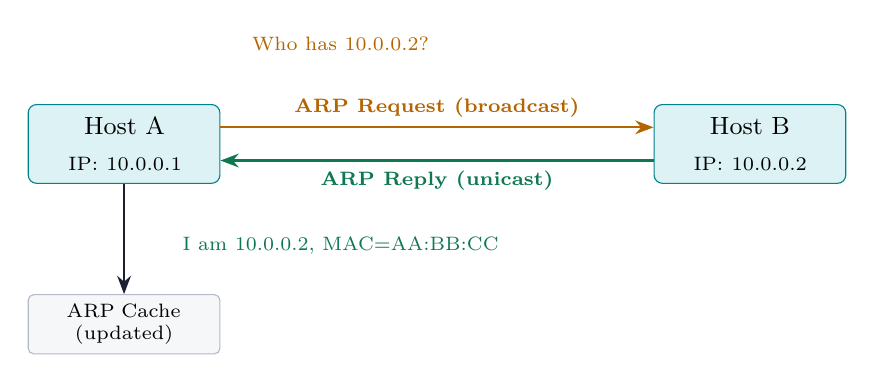
\begin{tikzpicture}[
  dev/.style={rectangle, draw=myteal, fill=hdrteal, text width=2.2cm, align=center, minimum height=1.0cm, font=\small, rounded corners=3pt},
  node distance=0.6cm
]
\node[dev] (A) {Host A\\[2pt]{\scriptsize IP: 10.0.0.1}};
\node[dev, right=5.5cm of A] (B) {Host B\\[2pt]{\scriptsize IP: 10.0.0.2}};

% ARP Request — above, with label above the arrow
\draw[-Stealth, thick, color=myamber]
  ([yshift=6pt]A.east) -- ([yshift=6pt]B.west)
  node[midway, above, font=\scriptsize\bfseries\color{myamber}] {ARP Request (broadcast)};
\node[font=\scriptsize\color{myamber}, above=0.55cm of A, xshift=2.75cm]
  {Who has 10.0.0.2?};

% ARP Reply — below, with label below the arrow
\draw[-Stealth, thick, color=mygreen]
  ([yshift=-6pt]B.west) -- ([yshift=-6pt]A.east)
  node[midway, below, font=\scriptsize\bfseries\color{mygreen}] {ARP Reply (unicast)};
\node[font=\scriptsize\color{mygreen}, below=0.55cm of A, xshift=2.75cm]
  {I am 10.0.0.2, MAC=AA:BB:CC};

% Cache
\node[rectangle, draw=mgframe, fill=mygray, text width=2.2cm, align=center,
  font=\scriptsize, below=1.4cm of A, rounded corners=2pt] (cache) {ARP Cache\\(updated)};
\draw[arrow] (A.south) -- (cache.north);
\end{tikzpicture}
\end{tcolorbox}

\textbf{IPv4 vs.\ IPv6 Key Differences:}\par\noindent
\begin{tabularx}{\linewidth}{|B{3.0cm}|X|X|}
\hline
\multicolumn{1}{|>{\centering\arraybackslash}p{3.0cm}|}{\textbf{Feature}} &
\multicolumn{1}{>{\centering\arraybackslash}X|}{\textbf{\color{myteal}IPv4}} &
\multicolumn{1}{>{\centering\arraybackslash}X|}{\textbf{\color{myamber}IPv6}} \\
\hline
Address size    & 32 bits (4 bytes)             & 128 bits (16 bytes) \\
\hline
Notation        & Dotted decimal (x.x.x.x)      & Colon-hex (x:x:x:x:x:x:x:x) \\
\hline
Header size     & 20--60 bytes (variable)        & 40 bytes (fixed) \\
\hline
Fragmentation   & By routers and hosts           & By source host only \\
\hline
Checksum        & Present in header              & Removed (handled by upper layers) \\
\hline
Security        & Optional (IPSec)               & Mandatory (IPSec built-in) \\
\hline
\end{tabularx}

%═══════════════════════════════════════════════════════════════════════════════
\section{Transport Layer}
%═══════════════════════════════════════════════════════════════════════════════

\begin{tcolorbox}[defbox]
\textbf{Transport Layer (Layer 4):} Provides \textit{process-to-process} (end-to-end) delivery of data. Handles segmentation, reassembly, flow control, error control, and multiplexing using \textbf{port numbers}.
\end{tcolorbox}

\subsection{UDP (User Datagram Protocol)}

\begin{tcolorbox}[formulabox, title={\textbf{UDP --- Connectionless, Unreliable}}]
\textbf{Features:} No connection setup, no acknowledgement, no flow/error control. Minimal overhead.\\
\textbf{Header:} 8 bytes --- Source Port (16b) $|$ Destination Port (16b) $|$ Length (16b) $|$ Checksum (16b).\\
\textbf{Use cases:} DNS, DHCP, SNMP, VoIP, video streaming, online gaming.\\
\textbf{Advantage:} Very fast, low latency. \textbf{Disadvantage:} No reliability guarantee.
\end{tcolorbox}

\subsection{TCP (Transmission Control Protocol)}

\begin{tcolorbox}[formulabox, title={\textbf{TCP --- Connection-Oriented, Reliable}}]
\textbf{Features:} Full-duplex, byte-stream, reliable delivery, flow control (sliding window), congestion control, ordered delivery.\\
\textbf{Header:} 20--60 bytes. Key fields: Source/Dest Port, Sequence No., ACK No., Flags (SYN, ACK, FIN, RST), Window Size, Checksum.\\
\textbf{Use cases:} HTTP, FTP, SMTP, SSH, Telnet.
\end{tcolorbox}

\textbf{TCP Three-Way Handshake (Connection Establishment):}
\begin{enumerate}[label=\textbf{\arabic*.}, leftmargin=*, itemsep=3pt]
  \item \textbf{SYN:} Client sends SYN segment with initial sequence number $x$.
  \item \textbf{SYN-ACK:} Server responds with SYN ($y$) + ACK ($x+1$).
  \item \textbf{ACK:} Client sends ACK ($y+1$). Connection established.
\end{enumerate}

\textbf{TCP Connection Termination (Four-Way):} FIN $\to$ ACK $\to$ FIN $\to$ ACK.

\begin{tcolorbox}[tikzbox, title={TCP Three-Way Handshake}]
\centering
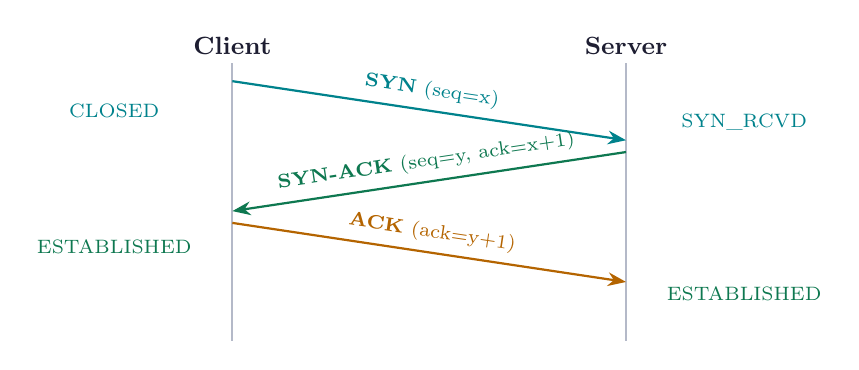
\begin{tikzpicture}[x=1cm, y=0.75cm,
  lbl/.style={font=\small\bfseries\color{mydark}},
  msg/.style={font=\scriptsize\color{mydark}}
]
\node[lbl] at (0,5.2) {Client};
\node[lbl] at (5,5.2) {Server};
\draw[thick,color=mgframe] (0,4.9) -- (0,0.2);
\draw[thick,color=mgframe] (5,4.9) -- (5,0.2);
% SYN
\draw[arrow,color=myteal] (0,4.6) -- node[above,sloped,msg]{\textbf{SYN} (seq=x)} (5,3.6);
\node[msg,color=myteal] at (-1.5,4.1) {CLOSED};
\node[msg,color=myteal] at (6.5,3.9) {SYN\_RCVD};
% SYN-ACK
\draw[arrow,color=mygreen] (5,3.4) -- node[above,sloped,msg]{\textbf{SYN-ACK} (seq=y, ack=x+1)} (0,2.4);
% ACK
\draw[arrow,color=myamber] (0,2.2) -- node[above,sloped,msg]{\textbf{ACK} (ack=y+1)} (5,1.2);
\node[msg,color=mygreen] at (-1.5,1.8) {ESTABLISHED};
\node[msg,color=mygreen] at (6.5,1.0) {ESTABLISHED};
\end{tikzpicture}
\end{tcolorbox}

\subsection{Congestion Control}

\begin{tcolorbox}[defbox]
\textbf{Congestion:} A state where the network cannot handle the offered load; routers drop packets, causing retransmissions and further congestion. Congestion control prevents/reduces this.
\end{tcolorbox}

\subsubsection*{Open Loop Congestion Control}
Prevents congestion \textbf{before it occurs} through good design policies:
\begin{itemize}[leftmargin=*, itemsep=3pt]
  \item \textbf{Retransmission policy:} Retransmit only when necessary (use timers wisely).
  \item \textbf{Window policy:} Use selective repeat (wastes less bandwidth than GBN).
  \item \textbf{Discarding policy:} Routers discard less sensitive packets first.
  \item \textbf{Acknowledgement policy:} Receiver delays ACK to reduce ACK traffic.
  \item \textbf{Admission policy:} Routers reject new connections if network is near capacity.
\end{itemize}

\subsubsection*{Closed Loop Congestion Control}
Reacts to congestion \textbf{after it occurs}:
\begin{itemize}[leftmargin=*, itemsep=3pt]
  \item \textbf{Backpressure:} Congested node sends a signal to upstream node to slow down. Works hop-by-hop.
  \item \textbf{Choke packet:} Congested router sends a choke packet directly to the source to reduce its transmission rate.
  \item \textbf{Implicit signalling:} Source detects congestion from dropped packets or increased delay (TCP's approach).
  \item \textbf{Explicit signalling:} Router sets a bit in the packet header to warn source/destination (ECN --- Explicit Congestion Notification).
\end{itemize}

\subsection{Quality of Service (QoS)}

\begin{tcolorbox}[defbox]
\textbf{QoS:} The ability of a network to provide different levels of service to different traffic types. Key metrics: \textbf{bandwidth}, \textbf{delay}, \textbf{jitter} (delay variation), \textbf{packet loss}.
\end{tcolorbox}

\subsubsection*{Leaky Bucket Algorithm}
\begin{tcolorbox}[formulabox, title={\textbf{Leaky Bucket Algorithm}}]
\textbf{Concept:} A bucket with a small hole at the bottom. Packets enter the bucket (queue) at any rate; they leave at a \textbf{constant rate} (the leak rate). Smooths bursty traffic into a steady stream.\\[4pt]
\textbf{Operation:}
\begin{itemize}[leftmargin=*, itemsep=2pt, topsep=0pt]
  \item If bucket is not full: incoming packet is added to the queue.
  \item If bucket is full: packet is \textbf{discarded} (overflow).
  \item Packets leave the bucket at a fixed rate $r$ (tokens/second).
\end{itemize}
\textbf{Advantage:} Enforces constant output rate. \textbf{Disadvantage:} Cannot handle bursts; excess packets dropped.
\end{tcolorbox}

\begin{tcolorbox}[tikzbox, title={Leaky Bucket vs Token Bucket}]
\centering
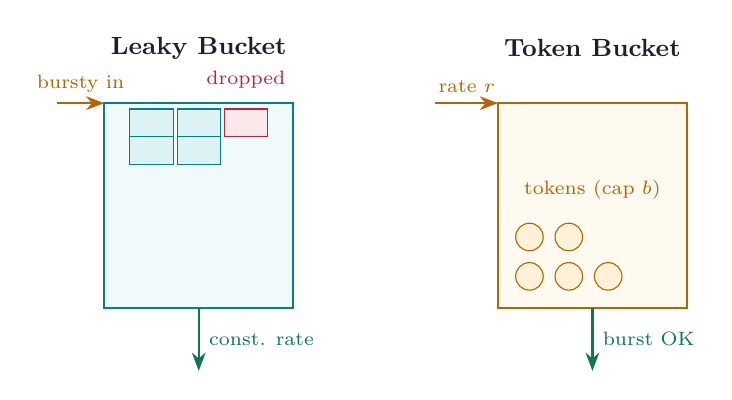
\begin{tikzpicture}[
  pkt/.style={rectangle, draw=myteal, fill=hdrteal, minimum width=0.55cm, minimum height=0.35cm, font=\tiny},
  tok/.style={circle, draw=myamber, fill=hdramber, minimum size=0.35cm, font=\tiny},
  lbl/.style={font=\small\bfseries\color{mydark}}
]
%--- Leaky Bucket (left) ---
\node[lbl] at (1.5,4.5) {Leaky Bucket};
% bucket outline
\draw[thick,color=myteal,fill=hdrteal!40] (0.3,1.2) -- (0.3,3.8) -- (2.7,3.8) -- (2.7,1.2) -- cycle;
% packets entering (bursty)
\foreach \y in {3.2,3.55} { \node[pkt] at (0.9,\y) {}; }
\foreach \y in {3.2,3.55} { \node[pkt] at (1.5,\y) {}; }
\node[pkt,draw=myred,fill=hdrred] at (2.1,3.55) {};
\node[font=\scriptsize\color{myred}] at (2.1,4.1) {dropped};
% arrows in
\draw[arrow,color=myamber] (-0.3,3.8) -- node[above]{\scriptsize bursty in} (0.3,3.8);
% hole at bottom
\draw[thick,color=myteal] (1.3,1.2) -- (1.7,1.2);
\draw[arrow,color=mygreen] (1.5,1.2) -- node[right]{\scriptsize const. rate} (1.5,0.4);

%--- Token Bucket (right) ---
\node[lbl] at (6.5,4.5) {Token Bucket};
\draw[thick,color=myamber,fill=hdramber!40] (5.3,1.2) -- (5.3,3.8) -- (7.7,3.8) -- (7.7,1.2) -- cycle;
% tokens
\foreach \x/\y in {5.7/1.6, 6.2/1.6, 6.7/1.6, 5.7/2.1, 6.2/2.1} { \node[tok] at (\x,\y) {}; }
\node[font=\scriptsize\color{myamber}] at (6.5,2.7) {tokens (cap $b$)};
% token generator
\draw[arrow,color=myamber] (4.5,3.8) -- node[above]{\scriptsize rate $r$} (5.3,3.8);
% packet consumes token
\draw[arrow,color=mygreen] (6.5,1.2) -- node[right]{\scriptsize burst OK} (6.5,0.4);
\end{tikzpicture}
\end{tcolorbox}

\subsubsection*{Token Bucket Algorithm}
\begin{tcolorbox}[formulabox, title={\textbf{Token Bucket Algorithm}}]
\textbf{Concept:} Tokens are generated at a constant rate $r$ and stored in a bucket (capacity $b$). A packet can only be sent if a token is available (one token consumed per packet).\\[4pt]
\textbf{Operation:}
\begin{itemize}[leftmargin=*, itemsep=2pt, topsep=0pt]
  \item Tokens accumulate up to bucket capacity $b$.
  \item To send a packet: remove one token from bucket.
  \item If no token available: packet must wait (or be discarded).
\end{itemize}
\textbf{Maximum burst size:} $b$ packets (when bucket is full).\\
\textbf{Advantage:} Allows controlled bursts up to $b$. More flexible than leaky bucket.
\end{tcolorbox}

\begin{tabularx}{\linewidth}{|B{3.0cm}|X|X|}
\hline
\multicolumn{1}{|>{\centering\arraybackslash}p{3.0cm}|}{\textbf{Feature}} &
\multicolumn{1}{>{\centering\arraybackslash}X|}{\textbf{\color{myteal}Leaky Bucket}} &
\multicolumn{1}{>{\centering\arraybackslash}X|}{\textbf{\color{myamber}Token Bucket}} \\
\hline
Output rate     & Constant (fixed)              & Variable (up to burst limit) \\
\hline
Burst handling  & Excess packets dropped        & Bursts allowed up to $b$ tokens \\
\hline
Flexibility     & Less flexible                 & More flexible \\
\hline
Use case        & Traffic shaping               & Traffic policing with burst allowance \\
\hline
\end{tabularx}

%═══════════════════════════════════════════════════════════════════════════════
% QUICK REVISION PAGE
%═══════════════════════════════════════════════════════════════════════════════
\newpage
\begin{center}
  {\large\bfseries\color{myred} Quick Revision --- Module 3}\\[3pt]
  {\small\color{mydark} Network Layer \& Transport Layer $|$ EC602}
\end{center}
\noindent{\color{myred}\rule{\linewidth}{1.2pt}}
\vspace{4pt}

\begin{tcolorbox}[formulabox, title={\textbf{Key Facts at a Glance}}]
\begin{tabularx}{\linewidth}{B{5.0cm} X}
Class A range           & 1--126; mask 255.0.0.0 \\[2pt]
Class B range           & 128--191; mask 255.255.0.0 \\[2pt]
Class C range           & 192--223; mask 255.255.255.0 \\[2pt]
Subnets                 & $2^s$ (s = borrowed bits) \\[2pt]
Hosts per subnet        & $2^h - 2$ (h = host bits) \\[2pt]
RIP metric / max hops   & Hop count / 15 \\[2pt]
OSPF metric             & Cost (bandwidth-based) \\[2pt]
BGP use                 & Inter-AS routing; TCP port 179 \\[2pt]
ARP function            & IP $\to$ MAC address resolution \\[2pt]
ICMP use                & Error reporting; ping (Echo Request/Reply) \\[2pt]
IPv6 address size       & 128 bits \\[2pt]
TCP handshake           & SYN $\to$ SYN-ACK $\to$ ACK \\[2pt]
UDP header size         & 8 bytes \\[2pt]
TCP header size         & 20--60 bytes \\[2pt]
Leaky bucket output     & Constant rate \\[2pt]
Token bucket burst      & Up to $b$ tokens \\[2pt]
\end{tabularx}
\end{tcolorbox}

\vspace{6pt}

\begin{tcolorbox}[defbox, title={\textbf{One-Line Definitions}}]
\begin{itemize}[leftmargin=*, itemsep=3pt, topsep=0pt]
  \item \textbf{Router:} Layer 3 device that routes packets between networks using IP addresses.
  \item \textbf{Gateway:} Protocol converter connecting networks with different protocols.
  \item \textbf{Subnetting:} Dividing a network into smaller subnets by borrowing host bits.
  \item \textbf{RIP:} Distance vector routing protocol; metric = hop count; max 15 hops.
  \item \textbf{OSPF:} Link state routing protocol; uses Dijkstra's algorithm; metric = cost.
  \item \textbf{BGP:} Path vector protocol for inter-AS routing on the Internet.
  \item \textbf{ARP:} Resolves IP address to MAC address via broadcast.
  \item \textbf{ICMP:} Reports network errors and provides diagnostic functions (ping).
  \item \textbf{TCP:} Reliable, connection-oriented transport protocol with flow/error control.
  \item \textbf{UDP:} Unreliable, connectionless transport protocol; low overhead, fast.
  \item \textbf{Congestion:} Network overload causing packet drops and retransmissions.
  \item \textbf{Leaky Bucket:} Traffic shaping algorithm enforcing constant output rate.
  \item \textbf{Token Bucket:} Traffic policing algorithm allowing controlled bursts.
\end{itemize}
\end{tcolorbox}

\vspace{6pt}

\begin{tcolorbox}[exambox, title={\textbf{Frequently Asked / Viva Questions}}]
\begin{enumerate}[leftmargin=*, topsep=0pt, label=\textbf{Q\arabic*.}, itemsep=8pt]
  \item \Q{What is the difference between a switch and a router?} Switch operates at Layer 2 (MAC addresses, within a network); router operates at Layer 3 (IP addresses, between networks).
  \item \Q{What is subnetting and why is it used?} Dividing a network into smaller subnets. Used to reduce broadcast domains, improve security, and efficient IP address utilisation.
  \item \Q{How many hosts can a /26 subnet support?} $2^6 - 2 = 62$ usable hosts.
  \item \Q{Difference between RIP and OSPF?} RIP: distance vector, hop count metric, max 15 hops, slow convergence. OSPF: link state, cost metric, no hop limit, fast convergence.
  \item \Q{What is BGP used for?} Inter-domain routing between Autonomous Systems on the Internet; uses path vector algorithm.
  \item \Q{What does ARP do?} Resolves an IP address to a MAC address by broadcasting an ARP request on the local network.
  \item \Q{Difference between TCP and UDP?} TCP: reliable, connection-oriented, ordered, flow/error control. UDP: unreliable, connectionless, no ordering, minimal overhead.
  \item \Q{What is the TCP three-way handshake?} SYN (client) $\to$ SYN-ACK (server) $\to$ ACK (client). Establishes a reliable connection.
  \item \Q{What is the difference between leaky bucket and token bucket?} Leaky bucket: constant output rate, excess dropped. Token bucket: variable output up to burst size $b$, more flexible.
  \item \Q{What is a choke packet?} A packet sent by a congested router directly to the source to reduce its transmission rate (closed-loop congestion control).
  \item \Q{What is the purpose of TTL in IP header?} Time To Live; decremented by each router. When TTL = 0, packet is discarded. Prevents infinite routing loops.
  \item \Q{What are the main improvements of IPv6 over IPv4?} 128-bit addressing, fixed 40-byte header, no router fragmentation, built-in IPSec, no broadcast (uses multicast).
\end{enumerate}
\end{tcolorbox}


% -- Module 4 -----------------------------------------------------------------
\modulestart{4}{Application Layer Protocols}

\section{Application Layer Protocols}
%═══════════════════════════════════════════════════════════════════════════════

\begin{tcolorbox}[defbox]
\textbf{Application Layer (Layer 7):} Provides network services directly to user applications. Protocols define the format and rules for communication between applications on different hosts.
\end{tcolorbox}

\begin{tabularx}{\linewidth}{|B{2.4cm}|>{\centering\arraybackslash}p{1.8cm}|>{\centering\arraybackslash}p{2.0cm}|X|}
\hline
\multicolumn{1}{|>{\centering\arraybackslash}p{2.4cm}|}{\textbf{\color{myteal}Protocol}} &
\textbf{\color{myteal}Port} &
\textbf{\color{myteal}Transport} &
\multicolumn{1}{>{\centering\arraybackslash}X|}{\textbf{\color{myteal}Function}} \\
\hline
DNS  & 53  & UDP/TCP & Resolves domain names to IP addresses. \\
\hline
SMTP & 25  & TCP     & Sends email from client to server (or server to server). \\
\hline
SNMP & 161 & UDP     & Manages and monitors network devices. \\
\hline
FTP  & 20/21 & TCP   & File transfer; port 21 = control, port 20 = data. \\
\hline
HTTP & 80  & TCP     & Transfers web pages (HyperText Transfer Protocol). \\
\hline
HTTPS& 443 & TCP     & Secure HTTP using TLS/SSL encryption. \\
\hline
\end{tabularx}

\subsection{DNS (Domain Name System)}

\begin{tcolorbox}[formulabox, title={\textbf{DNS}}]
\textbf{Function:} Translates human-readable domain names (e.g.\ \texttt{www.google.com}) to IP addresses.\\
\textbf{Hierarchy:} Root DNS $\to$ TLD servers (.com, .org, .in) $\to$ Authoritative DNS servers.\\
\textbf{Resolution types:}
\begin{itemize}[leftmargin=*, itemsep=2pt, topsep=0pt]
  \item \textbf{Recursive:} DNS resolver queries on behalf of client until answer found.
  \item \textbf{Iterative:} DNS server returns best referral; client queries next server itself.
\end{itemize}
\textbf{Caching:} DNS responses cached with TTL to reduce lookup time.
\end{tcolorbox}

\begin{tcolorbox}[tikzbox, title={DNS Resolution Hierarchy}]
\centering
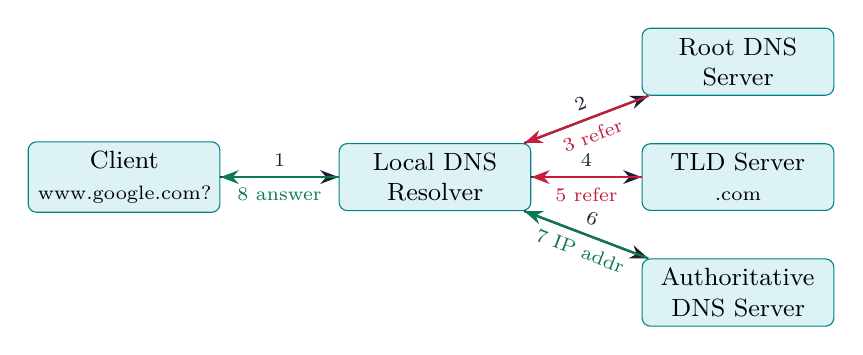
\begin{tikzpicture}[
  srv/.style={rectangle, draw=myteal, fill=hdrteal, text width=2.2cm, align=center, minimum height=0.65cm, font=\small, rounded corners=3pt},
  node distance=0.5cm
]
\node[srv] (client) {Client\\{\scriptsize www.google.com?}};
\node[srv, right=1.5cm of client] (resolver) {Local DNS\\Resolver};
\node[srv, above right=0.6cm and 1.4cm of resolver] (root) {Root DNS\\Server};
\node[srv, right=1.4cm of resolver] (tld) {TLD Server\\{\scriptsize .com}};
\node[srv, below right=0.6cm and 1.4cm of resolver] (auth) {Authoritative\\DNS Server};

\draw[arrow] (client) -- node[above]{\scriptsize 1} (resolver);
\draw[arrow] (resolver) -- node[above,sloped]{\scriptsize 2} (root);
\draw[arrow,color=myred] (root) -- node[below,sloped]{\scriptsize 3 refer} (resolver);
\draw[arrow] (resolver) -- node[above]{\scriptsize 4} (tld);
\draw[arrow,color=myred] (tld) -- node[below]{\scriptsize 5 refer} (resolver);
\draw[arrow] (resolver) -- node[above,sloped]{\scriptsize 6} (auth);
\draw[arrow,color=mygreen] (auth) -- node[below,sloped]{\scriptsize 7 IP addr} (resolver);
\draw[arrow,color=mygreen] (resolver) -- node[below]{\scriptsize 8 answer} (client);
\end{tikzpicture}
\end{tcolorbox}

\subsection{HTTP and WWW}

\begin{tcolorbox}[defbox]
\textbf{HTTP (HyperText Transfer Protocol):} Application layer protocol for transferring web content. Stateless, request-response model. Client sends HTTP request; server responds with status code and content.
\end{tcolorbox}

\textbf{HTTP Methods:} GET (retrieve), POST (submit data), PUT (update), DELETE (remove), HEAD (headers only).\\
\textbf{Common Status Codes:} 200 OK, 301 Moved Permanently, 404 Not Found, 500 Internal Server Error.\\
\textbf{WWW:} World Wide Web --- a system of interlinked hypertext documents accessed via HTTP. Uses URLs, HTML, and browsers.

%═══════════════════════════════════════════════════════════════════════════════
\section{Network Security}
%═══════════════════════════════════════════════════════════════════════════════

\subsection{Cryptography}

\begin{tcolorbox}[defbox]
\textbf{Cryptography:} The science of securing information by transforming it into an unreadable format (ciphertext) using an algorithm and a key. Only authorised parties with the correct key can decrypt it.
\end{tcolorbox}

\subsubsection*{Symmetric Key (Private Key) Cryptography}
\begin{tcolorbox}[formulabox, title={\textbf{Symmetric Key Cryptography}}]
\textbf{Concept:} Same key used for both encryption and decryption. Both sender and receiver must share the secret key securely.\\[4pt]
\textbf{Algorithms:} DES (56-bit key), 3DES, AES (128/192/256-bit), RC4, Blowfish.\\[4pt]
\textbf{Advantages:} Fast, low computational overhead, suitable for bulk data encryption.\\
\textbf{Disadvantages:} Key distribution problem --- how to securely share the key? Does not scale well ($n$ users need $n(n-1)/2$ keys).
\end{tcolorbox}

\subsubsection*{Asymmetric Key (Public Key) Cryptography}
\begin{tcolorbox}[formulabox, title={\textbf{Asymmetric Key Cryptography}}]
\textbf{Concept:} Uses a \textbf{key pair} --- a \textbf{public key} (shared openly) and a \textbf{private key} (kept secret). Data encrypted with public key can only be decrypted with the corresponding private key.\\[4pt]
\textbf{Algorithms:} RSA, Diffie-Hellman, ECC (Elliptic Curve Cryptography).\\[4pt]
\textbf{Encryption:} Sender encrypts with receiver's \textbf{public key}; receiver decrypts with \textbf{private key}.\\
\textbf{Advantages:} Solves key distribution problem; enables digital signatures.\\
\textbf{Disadvantages:} Computationally expensive; much slower than symmetric encryption.
\end{tcolorbox}

\begin{tabularx}{\linewidth}{|B{3.0cm}|X|X|}
\hline
\multicolumn{1}{|>{\centering\arraybackslash}p{3.0cm}|}{\textbf{Feature}} &
\multicolumn{1}{>{\centering\arraybackslash}X|}{\textbf{\color{myteal}Symmetric}} &
\multicolumn{1}{>{\centering\arraybackslash}X|}{\textbf{\color{myamber}Asymmetric}} \\
\hline
Keys used       & Same key (shared secret)      & Public + Private key pair \\
\hline
Speed           & Fast                          & Slow \\
\hline
Key distribution& Difficult (must share secretly)& Easy (public key is open) \\
\hline
Scalability     & Poor ($n^2/2$ keys)           & Good ($2n$ keys for $n$ users) \\
\hline
Examples        & AES, DES, RC4                 & RSA, Diffie-Hellman, ECC \\
\hline
Use case        & Bulk data encryption          & Key exchange, digital signatures \\
\hline
\end{tabularx}

\subsection{Digital Signature}

\begin{tcolorbox}[defbox]
\textbf{Digital Signature:} A cryptographic mechanism that provides \textbf{authentication}, \textbf{integrity}, and \textbf{non-repudiation}. Created by encrypting a message digest (hash) with the sender's \textbf{private key}.
\end{tcolorbox}

\textbf{Process:}
\begin{enumerate}[label=\textbf{\arabic*.}, leftmargin=*, itemsep=3pt]
  \item Sender computes hash of message using a hash function (e.g.\ SHA-256).
  \item Sender encrypts the hash with their \textbf{private key} --- this is the digital signature.
  \item Receiver decrypts the signature using sender's \textbf{public key} to get the hash.
  \item Receiver independently computes hash of received message.
  \item If both hashes match: message is authentic and unaltered.
\end{enumerate}

\begin{tcolorbox}[tikzbox, title={Digital Signature --- Sign \& Verify}]
\centering
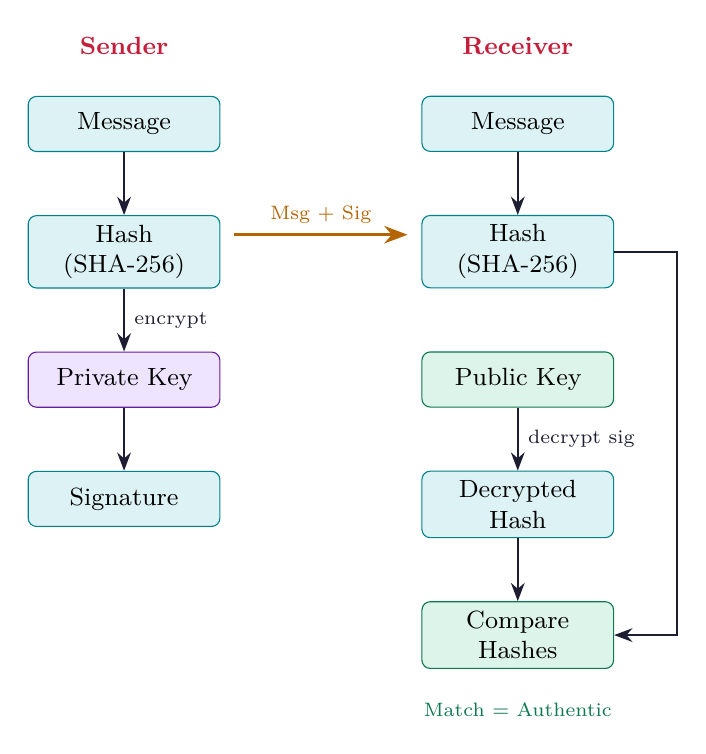
\begin{tikzpicture}[
  proc/.style={rectangle, draw=myteal, fill=hdrteal, text width=2.2cm, align=center, minimum height=0.7cm, font=\small, rounded corners=3pt},
  pkey/.style={rectangle, draw=mypurple, fill=hdrpurple, text width=2.2cm, align=center, minimum height=0.7cm, font=\small, rounded corners=3pt},
  gkey/.style={rectangle, draw=mygreen, fill=hdrgreen, text width=2.2cm, align=center, minimum height=0.7cm, font=\small, rounded corners=3pt},
  arr/.style={-Stealth, thick, color=mydark}
]
%--- SENDER column ---
\node[font=\small\bfseries\color{myred}] (slbl) at (1.1, 0.0) {Sender};
\node[proc,  below=0.4cm of slbl]  (msg1)  {Message};
\node[proc,  below=0.8cm of msg1]  (hash1) {Hash (SHA-256)};
\node[pkey,  below=0.8cm of hash1] (priv)  {Private Key};
\node[proc,  below=0.8cm of priv]  (sig)   {Signature};
\draw[arr] (msg1)  -- (hash1);
\draw[arr] (hash1) -- node[right, font=\scriptsize] {encrypt} (priv);
\draw[arr] (priv)  -- (sig);

%--- transfer arrow (horizontal, between columns) ---
\draw[-Stealth, very thick, color=myamber]
  (2.5, -2.4) -- node[above, font=\scriptsize\color{myamber}] {Msg + Sig} (4.7, -2.4);

%--- RECEIVER column ---
\node[font=\small\bfseries\color{myred}] (rlbl) at (6.1, 0.0) {Receiver};
\node[proc,  below=0.4cm of rlbl]  (msg2)  {Message};
\node[proc,  below=0.8cm of msg2]  (hash2) {Hash (SHA-256)};
\node[gkey,  below=0.8cm of hash2] (pub)   {Public Key};
\node[proc,  below=0.8cm of pub]   (dhash) {Decrypted Hash};
\node[gkey,  below=0.8cm of dhash] (cmp)   {Compare Hashes};
\draw[arr] (msg2)  -- (hash2);
\draw[arr] (pub)   -- node[right, font=\scriptsize] {decrypt sig} (dhash);
\draw[arr] (dhash) -- (cmp);
% hash2 feeds into compare via right side detour
\draw[arr] (hash2.east) -- ++(0.8,0) |- (cmp.east);

\node[font=\scriptsize\color{mygreen}, below=0.3cm of cmp] {Match = Authentic};
\end{tikzpicture}
\end{tcolorbox}

\subsection{Firewalls}

\begin{tcolorbox}[defbox]
\textbf{Firewall:} A network security device (hardware or software) that monitors and controls incoming/outgoing network traffic based on predefined security rules. Acts as a barrier between trusted internal network and untrusted external network.
\end{tcolorbox}

\textbf{Types of Firewalls:}\par\noindent
\begin{tabularx}{\linewidth}{|B{3.2cm}|X|}
\hline
\multicolumn{1}{|>{\centering\arraybackslash}p{3.2cm}|}{\textbf{\color{mygreen}Type}} &
\multicolumn{1}{>{\centering\arraybackslash}X|}{\textbf{\color{mygreen}Description}} \\
\hline
Packet Filter      & Inspects packets at network layer; filters based on IP, port, protocol. Stateless. \\
\hline
Stateful Inspection& Tracks connection state; allows only packets belonging to established connections. \\
\hline
Application Gateway& Proxy-based; inspects application layer data (HTTP, FTP). Most secure but slowest. \\
\hline
Circuit-level Gateway & Monitors TCP handshake; does not inspect packet content. \\
\hline
\end{tabularx}

\begin{tcolorbox}[tikzbox, title={Firewall Placement in a Network}]
\centering
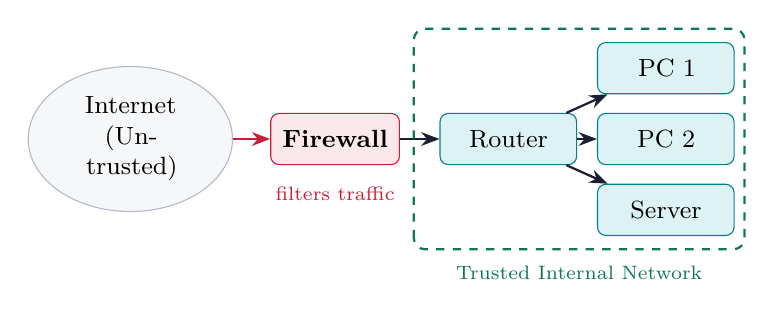
\begin{tikzpicture}[
  dev/.style={rectangle, draw=myteal, fill=hdrteal, text width=1.5cm, align=center, minimum height=0.65cm, font=\small, rounded corners=3pt},
  fw/.style={rectangle, draw=myred, fill=hdrred, text width=1.4cm, align=center, minimum height=0.65cm, font=\small\bfseries, rounded corners=3pt},
  cloud/.style={ellipse, draw=mgframe, fill=mygray, text width=1.6cm, align=center, font=\small}
]
\node[cloud] (inet)   at (0, 0)    {Internet\\(Untrusted)};
\node[fw]    (fw)     at (2.6, 0)  {Firewall};
\node[dev]   (router) at (4.8, 0)  {Router};
\node[dev]   (pc1)    at (6.8, 0.9){PC 1};
\node[dev]   (pc2)    at (6.8, 0)  {PC 2};
\node[dev]   (server) at (6.8,-0.9){Server};

\draw[arrow, color=myred] (inet)   -- (fw);
\draw[arrow]              (fw)     -- (router);
\draw[arrow]              (router) -- (pc1);
\draw[arrow]              (router) -- (pc2);
\draw[arrow]              (router) -- (server);

% dashed trusted zone box
\draw[dashed, color=mygreen, thick, rounded corners=4pt]
  (3.6, -1.4) rectangle (7.8, 1.4);
\node[font=\scriptsize\color{mygreen}] at (5.7, -1.7) {Trusted Internal Network};

% firewall label below fw node
\node[font=\scriptsize\color{myred}, below=0.15cm of fw] {filters traffic};
\end{tikzpicture}
\end{tcolorbox}

%═══════════════════════════════════════════════════════════════════════════════
\section{Modern Topics}
%═══════════════════════════════════════════════════════════════════════════════

\subsection{ISDN (Integrated Services Digital Network)}

\begin{tcolorbox}[defbox]
\textbf{ISDN:} A set of communication standards for simultaneous digital transmission of voice, video, data, and other services over traditional telephone copper wire. Replaced by DSL and broadband.
\end{tcolorbox}

\textbf{ISDN Channels:}
\begin{itemize}[leftmargin=*, itemsep=3pt]
  \item \textbf{B channel (Bearer):} 64 Kbps; carries user data (voice, video, data).
  \item \textbf{D channel (Delta):} 16 or 64 Kbps; carries signalling and control information.
\end{itemize}

\textbf{ISDN Interfaces:}\par\noindent
\begin{tabularx}{\linewidth}{|B{2.8cm}|X|}
\hline
\multicolumn{1}{|>{\centering\arraybackslash}p{2.8cm}|}{\textbf{\color{myteal}Interface}} &
\multicolumn{1}{>{\centering\arraybackslash}X|}{\textbf{\color{myteal}Description}} \\
\hline
BRI (Basic Rate)   & $2B + D$ = $2 \times 64$ Kbps + 16 Kbps D = 144 Kbps. For home/small office. \\
\hline
PRI (Primary Rate) & $23B + D$ (North America) or $30B + D$ (Europe) = 1.544 / 2.048 Mbps. For enterprises. \\
\hline
\end{tabularx}

\subsection{ATM (Asynchronous Transfer Mode)}

\begin{tcolorbox}[defbox]
\textbf{ATM:} A cell-switching and multiplexing technology that uses fixed-size \textbf{53-byte cells} (5-byte header + 48-byte payload) for transmitting voice, video, and data over high-speed networks.
\end{tcolorbox}

\textbf{Key Features:}
\begin{itemize}[leftmargin=*, itemsep=3pt]
  \item Fixed 53-byte cells enable predictable, low-latency switching.
  \item Connection-oriented: virtual circuits (VC) established before data transfer.
  \item Supports QoS guarantees for different traffic types (CBR, VBR, ABR, UBR).
  \item \textbf{VPI/VCI:} Virtual Path Identifier / Virtual Channel Identifier used for routing cells.
\end{itemize}

\subsection{DSL (Digital Subscriber Line)}

\begin{tcolorbox}[defbox]
\textbf{DSL:} A family of technologies that transmit digital data over existing telephone copper wire pairs at high speeds. Uses frequencies above the voice band (above 4 kHz).
\end{tcolorbox}

\begin{tabularx}{\linewidth}{|B{2.8cm}|X|X|}
\hline
\multicolumn{1}{|>{\centering\arraybackslash}p{2.8cm}|}{\textbf{Type}} &
\multicolumn{1}{>{\centering\arraybackslash}X|}{\textbf{Speed}} &
\multicolumn{1}{>{\centering\arraybackslash}X|}{\textbf{Description}} \\
\hline
ADSL (Asymmetric)  & Down: 8 Mbps, Up: 1 Mbps & Different download/upload speeds. Most common for home use. \\
\hline
SDSL (Symmetric)   & 2 Mbps both ways          & Equal upload/download. Used by businesses. \\
\hline
VDSL (Very High)   & Down: 52 Mbps, Up: 16 Mbps & Very high speed over short distances. \\
\hline
\end{tabularx}

\textbf{DSL Modem:} Connects user's equipment to the telephone line. Separates voice (0--4 kHz) and data (above 4 kHz) using a \textbf{splitter}.

\subsection{Cable Modem}

\begin{tcolorbox}[defbox]
\textbf{Cable Modem:} A device that provides Internet access over the cable TV (CATV) infrastructure using coaxial cable. Uses \textbf{DOCSIS} (Data Over Cable Service Interface Specification) standard.
\end{tcolorbox}

\textbf{Key Points:}
\begin{itemize}[leftmargin=*, itemsep=3pt]
  \item Shared medium: all users in a neighbourhood share the same cable segment (bandwidth shared).
  \item Downstream (TV to user): 6 MHz channel, up to 30--40 Mbps.
  \item Upstream (user to TV headend): narrower band, typically 5--42 MHz.
  \item \textbf{HFC (Hybrid Fibre-Coaxial):} Fibre from headend to neighbourhood node; coaxial to homes.
\end{itemize}

\subsection{Wireless LAN --- IEEE 802.11}

\begin{tcolorbox}[defbox]
\textbf{IEEE 802.11 (Wi-Fi):} A set of standards for wireless local area networking. Uses radio frequencies (2.4 GHz and 5 GHz bands). MAC protocol: CSMA/CA.
\end{tcolorbox}

\textbf{IEEE 802.11 Standards:}\par\noindent
\begin{tabularx}{\linewidth}{|>{\centering\arraybackslash}p{2.0cm}|>{\centering\arraybackslash}p{2.0cm}|>{\centering\arraybackslash}p{2.4cm}|X|}
\hline
\textbf{\color{myteal}Standard} & \textbf{\color{myteal}Year} & \textbf{\color{myteal}Frequency} & \multicolumn{1}{>{\centering\arraybackslash}X|}{\textbf{\color{myteal}Max Speed}} \\
\hline
802.11b & 1999 & 2.4 GHz & 11 Mbps \\
\hline
802.11a & 1999 & 5 GHz   & 54 Mbps \\
\hline
802.11g & 2003 & 2.4 GHz & 54 Mbps \\
\hline
802.11n & 2009 & 2.4/5 GHz & 600 Mbps (MIMO) \\
\hline
802.11ac& 2013 & 5 GHz   & 1+ Gbps \\
\hline
\end{tabularx}

\textbf{Architecture:}
\begin{itemize}[leftmargin=*, itemsep=3pt]
  \item \textbf{Infrastructure mode:} Devices connect through an \textbf{Access Point (AP)}. AP connects to wired network. Most common.
  \item \textbf{Ad-hoc mode:} Devices communicate directly without an AP (peer-to-peer).
  \item \textbf{BSS (Basic Service Set):} Single AP + associated stations.
  \item \textbf{ESS (Extended Service Set):} Multiple BSSs connected via a distribution system.
\end{itemize}

\textbf{Security:} WEP (weak, deprecated) $\to$ WPA $\to$ WPA2 (AES-based, current standard) $\to$ WPA3.

\subsection{Bluetooth}

\begin{tcolorbox}[defbox]
\textbf{Bluetooth (IEEE 802.15.1):} A short-range wireless technology for personal area networks (PAN). Operates at 2.4 GHz ISM band. Range: $\sim$10 m (Class 2). Uses \textbf{FHSS} (Frequency Hopping Spread Spectrum) --- hops 1600 times/second across 79 channels.
\end{tcolorbox}

\textbf{Bluetooth Network (Piconet):}
\begin{itemize}[leftmargin=*, itemsep=3pt]
  \item \textbf{Piconet:} One \textbf{master} + up to 7 active \textbf{slaves}. Master controls timing and frequency hopping.
  \item \textbf{Scatternet:} Multiple overlapping piconets; a device can be slave in multiple piconets or master in one and slave in another.
\end{itemize}

\begin{tcolorbox}[tikzbox, title={Bluetooth Piconet Structure}]
\centering
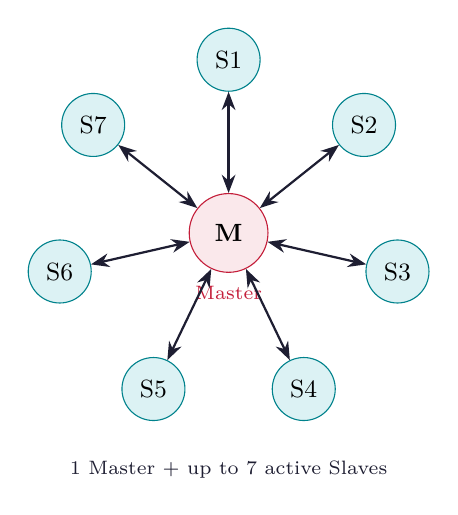
\begin{tikzpicture}[
  master/.style={circle, draw=myred, fill=hdrred, minimum size=1.0cm, font=\small\bfseries, align=center},
  slave/.style={circle, draw=myteal, fill=hdrteal, minimum size=0.8cm, font=\small, align=center}
]
\node[master] (M) {M};
\node[font=\scriptsize\color{myred}, below=0.05cm of M] {Master};
\foreach \i/\lbl in {1/S1, 2/S2, 3/S3, 4/S4, 5/S5, 6/S6, 7/S7} {
  \pgfmathsetmacro\ang{90 - (\i-1)*360/7}
  \node[slave] (S\i) at (\ang:2.2cm) {\lbl};
  \draw[thick, color=mydark, <->, >=Stealth] (M) -- (S\i);
}
\node[font=\scriptsize\color{mydark}] at (0,-3.0) {1 Master + up to 7 active Slaves};
\end{tikzpicture}
\end{tcolorbox}

\textbf{Bluetooth Versions:}\par\noindent
\begin{tabularx}{\linewidth}{|>{\centering\arraybackslash}p{2.2cm}|X|}
\hline
\textbf{\color{myteal}Version} & \multicolumn{1}{>{\centering\arraybackslash}X|}{\textbf{\color{myteal}Key Feature}} \\
\hline
1.2  & Basic rate 1 Mbps; AFH (Adaptive Frequency Hopping) \\
\hline
2.0 + EDR & Enhanced Data Rate; up to 3 Mbps \\
\hline
4.0 (BLE) & Bluetooth Low Energy; very low power; IoT devices \\
\hline
5.0  & 2$\times$ speed, 4$\times$ range, 8$\times$ broadcast capacity vs.\ 4.2 \\
\hline
\end{tabularx}

%═══════════════════════════════════════════════════════════════════════════════
% QUICK REVISION PAGE
%═══════════════════════════════════════════════════════════════════════════════
\newpage
\begin{center}
  {\large\bfseries\color{myred} Quick Revision --- Module 4}\\[3pt]
  {\small\color{mydark} Application Layer, Security \& Modern Topics $|$ EC602}
\end{center}
\noindent{\color{myred}\rule{\linewidth}{1.2pt}}
\vspace{4pt}

\begin{tcolorbox}[formulabox, title={\textbf{Key Facts at a Glance}}]
\begin{tabularx}{\linewidth}{B{5.0cm} X}
DNS port            & 53 (UDP/TCP) \\[2pt]
SMTP port           & 25 (TCP) \\[2pt]
FTP ports           & 21 (control), 20 (data) \\[2pt]
HTTP / HTTPS ports  & 80 / 443 \\[2pt]
SNMP port           & 161 (UDP) \\[2pt]
Symmetric key       & Same key for encrypt/decrypt (AES, DES) \\[2pt]
Asymmetric key      & Public key encrypts; private key decrypts (RSA) \\[2pt]
Digital signature   & Hash encrypted with sender's private key \\[2pt]
ISDN BRI            & $2B + D$ = 144 Kbps \\[2pt]
ISDN PRI (Europe)   & $30B + D$ = 2.048 Mbps \\[2pt]
ATM cell size       & 53 bytes (5 header + 48 payload) \\[2pt]
ADSL speed          & Down 8 Mbps / Up 1 Mbps \\[2pt]
802.11b speed       & 11 Mbps @ 2.4 GHz \\[2pt]
802.11g/a speed     & 54 Mbps \\[2pt]
Bluetooth range     & $\sim$10 m; 2.4 GHz; FHSS; 1600 hops/sec \\[2pt]
Piconet             & 1 master + up to 7 active slaves \\[2pt]
\end{tabularx}
\end{tcolorbox}

\vspace{6pt}

\begin{tcolorbox}[defbox, title={\textbf{One-Line Definitions}}]
\begin{itemize}[leftmargin=*, itemsep=3pt, topsep=0pt]
  \item \textbf{DNS:} Translates domain names to IP addresses using a hierarchical distributed database.
  \item \textbf{HTTP:} Stateless request-response protocol for transferring web content.
  \item \textbf{SMTP:} Protocol for sending email between mail servers.
  \item \textbf{FTP:} Protocol for transferring files; uses separate control (21) and data (20) connections.
  \item \textbf{Symmetric Cryptography:} Same secret key used for both encryption and decryption.
  \item \textbf{Asymmetric Cryptography:} Public key encrypts; private key decrypts (or vice versa for signatures).
  \item \textbf{Digital Signature:} Hash of message encrypted with sender's private key; proves authenticity.
  \item \textbf{Firewall:} Security device that filters network traffic based on rules.
  \item \textbf{ISDN:} Digital telephone network supporting voice, video, and data simultaneously.
  \item \textbf{ATM:} Cell-switching technology using fixed 53-byte cells; supports QoS.
  \item \textbf{DSL:} High-speed Internet over telephone copper wire using frequencies above voice band.
  \item \textbf{IEEE 802.11:} Wi-Fi standard; uses CSMA/CA; operates at 2.4/5 GHz.
  \item \textbf{Bluetooth:} Short-range PAN technology; 2.4 GHz; FHSS; piconet architecture.
\end{itemize}
\end{tcolorbox}

\vspace{6pt}

\begin{tcolorbox}[exambox, title={\textbf{Frequently Asked / Viva Questions}}]
\begin{enumerate}[leftmargin=*, topsep=0pt, label=\textbf{Q\arabic*.}, itemsep=8pt]
  \item \Q{What is DNS and how does it work?} DNS translates domain names to IP addresses. Client queries local DNS resolver; if not cached, resolver queries root $\to$ TLD $\to$ authoritative DNS servers recursively or iteratively.
  \item \Q{What is the difference between symmetric and asymmetric cryptography?} Symmetric: same key for encrypt/decrypt, fast, key distribution problem. Asymmetric: public/private key pair, slower, solves key distribution.
  \item \Q{How does a digital signature work?} Sender hashes the message and encrypts the hash with their private key. Receiver decrypts with sender's public key and compares hashes to verify authenticity and integrity.
  \item \Q{What is a firewall?} A security device that monitors and filters network traffic based on predefined rules, acting as a barrier between trusted and untrusted networks.
  \item \Q{What is the difference between packet filter and stateful firewall?} Packet filter: stateless, inspects each packet independently. Stateful: tracks connection state, allows only packets belonging to established connections.
  \item \Q{What is ATM and what is its cell size?} Asynchronous Transfer Mode; cell-switching technology using fixed 53-byte cells (5-byte header + 48-byte payload).
  \item \Q{What is ADSL?} Asymmetric DSL; provides higher download speed (up to 8 Mbps) than upload speed (up to 1 Mbps) over telephone copper wire.
  \item \Q{What MAC protocol does IEEE 802.11 use?} CSMA/CA (Carrier Sense Multiple Access with Collision Avoidance).
  \item \Q{What is a piconet in Bluetooth?} A small network of one master and up to 7 active slave devices communicating on the same frequency hopping sequence.
  \item \Q{What is FHSS in Bluetooth?} Frequency Hopping Spread Spectrum; Bluetooth hops across 79 channels 1600 times per second to reduce interference and improve security.
  \item \Q{What is the difference between infrastructure and ad-hoc Wi-Fi mode?} Infrastructure: devices connect through an Access Point. Ad-hoc: devices communicate directly without an AP.
  \item \Q{What is ISDN BRI?} Basic Rate Interface: $2B + D$ channels = $2 \times 64$ Kbps + 16 Kbps = 144 Kbps total. Used for home/small office ISDN connections.
\end{enumerate}
\end{tcolorbox}

\vspace{6pt}

\begin{tcolorbox}[tikzbox, title={\textbf{Application Layer Protocols Summary}}]
\begin{tabularx}{\linewidth}{|B{2.4cm}|>{\centering\arraybackslash}p{1.6cm}|>{\centering\arraybackslash}p{1.8cm}|X|}
\hline
\textbf{Protocol} & \textbf{Port} & \textbf{Transport} & \textbf{Purpose} \\
\hline
DNS  & 53  & UDP/TCP & Name resolution \\
\hline
SMTP & 25  & TCP & Send email \\
\hline
FTP  & 20/21 & TCP & File transfer \\
\hline
HTTP & 80  & TCP & Web pages \\
\hline
HTTPS& 443 & TCP & Secure web \\
\hline
SNMP & 161 & UDP & Network management \\
\hline
\end{tabularx}
\end{tcolorbox}


\end{document}
